\documentclass{book}

\usepackage[includefoot]{geometry}
% define page size and margins etc
\geometry{paperwidth=8.5in,paperheight=11in,
%\geometry{paperwidth=18.91cm,paperheight=24.589cm,
vmargin=1.9cm, % top and bottom margins
inner=1.9cm, % inside margin
outer=2.29cm, % outside margin
bindingoffset=0.89cm % gutter
}


\usepackage{subfigure}
\usepackage[subfigure]{tocloft}

\usepackage{fancyhdr} % to format headers/footers

\pagestyle{fancy}

%% fiddle with chaptermark so we can make it not all caps
\renewcommand{\chaptermark}[1]{\markboth{#1}{}}
\renewcommand{\sectionmark}[1]{\markright{#1}{}}


% makes it so article sections continue through independent of chapters
\usepackage{remreset}

\makeatletter
  \@removefromreset{section}{chapter}
\makeatother

\renewcommand{\thesection}{Article \arabic{section}}
%\renewcommand{\thesubsection}{Text \arabic{section}}

%% next get rid of existing header and footer and header rule
\fancyhead{}
\fancyfoot{}
\renewcommand{\headrulewidth}{0pt}

% now make the footer the way we want it:
% page number on right side of footer for odd pages
\rfoot[]{\small{\textsf{\hspace{0.25cm} \thepage}}}
\fancyhfoffset[EL]{0cm} % this looks like it doesn't do anything, but
                        % it seems to remind it to line up headers with the
                        % rest of the text

% page number and chapter name on left side of footer for even pages
\lfoot[\small{\textsf{\thepage \hspace{0.25cm} \leftmark}}]{}


% enables valign adjustments
\usepackage[export]{adjustbox}% http://ctan.org/pkg/adjustbox

\fancyfoot[C]{
    \includegraphics[valign=c,width=0.045\textwidth]{images/USSSA_shield_white_border_300_dpi}
}


%\includegraphics[scale=0.22,valign=c]{example-image}}



\usepackage[hang,flushmargin]{footmisc}  % To not indent footnotes

\usepackage[T1]{fontenc}
\usepackage{tgtermes}    % body font
\usepackage{inconsolata} % fixed width font
\usepackage{tgheros}     % sans-serif font


\usepackage[small]{caption}  % make caption text size smaller



%% Make the space above and below captions smaller
\setlength{\abovecaptionskip}{1.2ex}
\setlength{\belowcaptionskip}{-1.5ex}


% set all section headers to be sans-serif
%\allsectionsfont{\normalfont\sffamily}

\newcounter{stronglevel}
\setcounter{stronglevel}{1}
\newcommand{\strong}[1]{%
    \csname strong\roman{stronglevel}\endcsname{{%
        \advance\value{stronglevel} by 1\relax
        #1%
    }}%
}
\newcommand{\strongi}[1]{\textbf{#1}}
\newcommand{\strongii}[1]{{\blendcolors*{!50!red}\color{.}#1}}
\newcommand{\strongiii}[1]{\textsf{#1}}
\newcommand{\strongiv}[1]{{\blendcolors*{!50!red}\color{.}#1}}

% make all verbatim (code blocks) text smaller, just because it was bugging me
\let\oldverbatim\verbatim
\renewcommand\verbatim{\small\oldverbatim}


% Table of contents packages and settings
\usepackage{tocloft}  % to typeset table of contents
\renewcommand{\cftchapfont}{\sffamily}     % set TOC entries to sserif
\renewcommand{\cftchappagefont}{\sffamily} % set TOC page numbers to sserif
\setlength{\cftsecnumwidth}{45pt}          % set TC spacing to accommodate 'Article'

% format title of TOC: make sure this matches chapter head format as set below
\renewcommand{\cfttoctitlefont}{\hfill\Huge\sffamily}

\setcounter{tocdepth}{1} % sets what level of header is shown in the TOC
\setcounter{secnumdepth}{2} % sets what level of subsect. are numbered


\usepackage{titlesec} % to format chapter title pages

% format chapter title pages
\titleformat{\chapter}
  [display] % shape/type of title
  {\ttfamily} % formatting commands applied to both label and title
  {\vspace{-2cm} \hfill \large [chapter\kern0.15em\thechapter]}
  {2cm} % separation between number and chapter title
  {\huge\sffamily} % code preceding title. Last cmd can take arg, which is title
  [  % everything inside [] comes after the title
     \Large % make text that follows large
     \thispagestyle{plain} % suppress page numbers
     \chapterauthor% insert chapter author name
  ]% end of what comes after title


\usepackage{enumitem}

\usepackage[hyphens]{url} % this package doesn't make proper clickable
                          % links, but
% \usepackage{hyperref} % this package breaks the build.


\usepackage{microtype}


\usepackage{amssymb}


\usepackage{sectsty}


\usepackage{mathtools} % for bmatrix in matplotlib


\usepackage{enumitem}  % to manage spacing in and around lists
% define a legal 1., 1.1, 1.1.1 list
\newlist{legal}{enumerate}{10}
\setlist[legal]{label*=\arabic*.}


\usepackage{multicol} % to break the list of reviewers into columns


\usepackage{epigraph} % for fancy quoting


\begin{document}


\frontmatter



\begin{titlepage}
\chapter*{Pencak Silat Rules \& Regulations}
\begin{center}
    \begin{figure*}[ht!]
    \subfigure{
        \includegraphics[height=2.75in]{images/persilat_logo}
    }
    ~
    \subfigure{
        \includegraphics[height=2.75in]{images/USSSA_shield_white_border_300_dpi}
    }
\end{figure*}
\end{center}

\noindent International Pencak Silat Competitions are performed in principles of brotherhood and knightly soul by using elements of self defense, arts and Pencak Silat sports and by highly honoring the PESILAT PLEDGE.\\

\noindent The competitions are carried out in accordance with the category rules regulated in the competition regulations and conducted by certified legal and valid technical official of competitions. \\

\noindent Pencak Silat competition categories consist of: \\
\begin{enumerate}
    \item TANDING (Sparring Match) category
    \item TUNGGAL (Solo Performance) category
    \item GANDA (Choreographed Pair Performance) category
    \item REGU (Synchronized Team Performance) category
\end{enumerate}

\noindent In order to conduct Pencak Silat competition at the highest standards possible and in compliance with 
their intended purposes and objectives, the Pencak Silat Rules and Regulation is established as detailed in this technical manual.
\end{titlepage}

\section*{PERSILAT}
The governing body for international pencak silat is the International Pencak Silat Association or PERSILAT (Persekutuan Pencak Silat Antara Bangsa).

\begin{table*}
\begin{tabular}{p{3in}p{3in}}
\emph{A Pesilat is a person of noble character.\newline
A Pesilat is a person who respects his neighbor and loves friendship and peace.\newline
A Pesilat is a person who always thinks and acts positively, creatively and dynamically.\newline
A Pesilat is a knight who upholds truth, honesty and justice and always perseveres in facing temptations and trials.
\newline
A Pesilat is a knight who always takes responsibility for his words and actions.
}
&
\emph{Pesilat adalah pribadi yang berbudi pekerti luhur.\newline
Pesilat adalah insan yang menghormati sesamanya serta mencintai persaha-batan dan perdamaian.\newline
Pesilat adalah insan yang selalu berpikir dan bertindak positif, kreatif dan dinamis.\newline
Pesilat adalah kesatria yang menegakkan kebenaran, kejujuran dan keadilan serta senantiasa tahan uji dalam mengha-dapi godaan dan cobaan.\newline
Pesilat adalah kesatria yang senantiasa mempertanggungjawabkan kata-kata dan perbuatannya.
} \\
& \\
& --PERSILAT Pledge
\end{tabular}
\end{table*}

\section*{USSSA}

The United States Sport Silat Association (USSSA) is the sole national body for Pencak Silat competition in the United States recognized by the International Pencak Silat Federation (PERSILAT).

The USSSA coordinates local, state and national level competitions, so that it may field a strong USA Pencak Silat National Team that represents the United States' diversity of talent, knowledge and skill in Pencak Silat.

\subsection*{Mission}
To share the cultural heritage of Pencak Silat and the Indo-Malay archipelago with all Americans.

\subsection*{Vision}
To serve as a beacon of Pencak Silat values through sport, fellowship and education.  To bring together Pencak Silat players from all geographies and background.  To foster goodwill with other countries through competition and the shared bond of Pencak Silat.



\tableofcontents

\mainmatter
\chapter{Competition Regulations}

\section{Definition of Each Category}

\begin{enumerate}
\item TANDING (Sparring Match) category is the category of Pencak Silat competition that confronts 2 (two) Pesilat from different teams. Both of them confront each other by using the elements of self-defence and attacking such as defending/avoiding/hitting/attacking the target and dropping the opponent; the use of competition techniques and tactics, stamina and endurance, and fighting spirit, using the principles and using the richness of movement of techniques.

\url{https://youtu.be/Sy1wCmHILnA}


TUNGGAL (Solo Performance) is the category of Pencak Silat competition performed by one Pesilat that performs his skill in Jurus Tunggal Baku (Solo Compulsory Movement), accurately and firmly, complete soulfully with empty hands and with weapons according to rules and regulations apply for Tunggal category.

\url{https://youtu.be/_fcd-27kMhE}

\item GANDA (Choreographed Pair Performance) is the category of Pencak Silat competition which features two Pesilat of the same team performs choreographed technical skills rich of attacking – defensive movement of Pencak Silat. The movement of the attacking-defensive movement is performed with a well planned, effective, aesthetical, powerful and in an orderly series, with empty hands or with weapon according to rules and regulations apply for Ganda category.

\url{https://youtu.be/eUsunr0dTKk}

\item REGU (Synchronized Team Performance) category is the category of Pencak Silat competition which is performed by 3 (three) Pesilat from the same team portraying their skills in a compulsory movements correctly, accurately, firmly, complete with expression, synchronize and compact with empty hands according to rules and regulations apply for Regu category 

\url{https://youtu.be/Q6JSm8Mcd4w}

\end{enumerate}



\section{Classification of Competitions and Regulation of Age, Gender and Weight}


\begin{legal}
\item The top-level classifications of Pencak Silat competitions according to age, gender and weight for all categories consist of:
    \begin{legal}
    \item USSSA / USA Youth
        \begin{legal}
        \item Competition of USA-JUNIOR-I for Male and Female aged 10 to 11 years.
        \item Competition of USA-JUNIOR-II for Male and Female aged 12 to 14 years.
        \item Competition of USA-JUNIOR-III for Male and Female aged 15 to 16 years.
        \end{legal}
    \item PERSILAT / International Youth
        \begin{legal}
        \item Competition of PRE-TEEN for Male and Female aged over 10 to 12 years.
        \item Competition of PRE-JUNIOR for Male and Female aged over 12 to 14 years.
        \item Competition of JUNIOR for Male and Female aged over 14 to 17 years
        \end{legal}
    \item Adult
        \begin{legal}
        \item Competition of SENIOR for Male and Female aged over 17 to 35 years.
        \item Competition of MASTER-I for Male and Female aged over 35 to 45 years
        \item Competition of MASTER-II for Male and Female aged over 45 years
        \end{legal}
    \end{legal}

\item Confirmation of the age and citizenship (refer to annex) of a Pesilat participating in Competition is proved by a birth certificate, diploma, original passport or certified true Copy documents.

\item The age of Pesilat must confirm with the classification of age of the participants on the first day of the competition (regardless of any competition category).

\item The classification of classes according to body weight is valid only for TANDING category which is performed by weighing in.

    \begin{legal}
    \item No tolerance of body weight.
    \item The weigh-in is carried out 15 (fifteen) minutes before the start of the match in one Championship according to the schedule of the competition.
During the weigh-in the Pesilat (contestant) must wear a Pencak Silat unform using for competition, dry, without sash, without groin guard or any joint guards.
    \item A Pesilat (contestant) whose weight fails to meet his/her class requirement during weigh-in will be disqualified from the competition.  
The weigh-in is only carried out once and must be witnessed by officials from both teams and a referee-jury on duty. 
    \item It is mandatory for the weigh-in officials and officials from both teams to sign the weigh-in form which is provided by the Organizing Committee. When one of the team officials failed to endorse the form them weigh-in remains valid.
    \item The weigh-in officials are appointed by the organizing committee.
    \end{legal}

\item Certification of Medical Checkup
    \begin{legal}
    \item Every Pesilat (contestant) should produce a certified medical certificate, i.e. a letter to prove good health issued by authorized doctor or hospital/clinic, 1 month maximum before the first of competition regardless of competition category. 
    \item A Pesilat (contestant) who failed to show the medical certification before weighing in will be disqualified from the competition. 
    \end{legal}
    Organizing committee may recommend a certain doctor/hospital in the hosting country/city where cost is borne by the team of Pesilat. 
\end{legal}


\section{Youth Classifications}

\begin{legal}
\item USSSA / Domestic Youth Classifications

For domestic competition, USSSA has established classifications to align with divisions and levels 
found in other youth sports and martial arts competitions in the United States.  These are referred to as USA JUNIOR I, II and III resepectively.  These three levels are further detailed in~\ref{sec:usa_junior}.

\item PERSILAT / International Youth Classifications

PERSILAT Youth Classes are used in international competition. For consistency with other
    PERSILAT member organizations, the same nomenclature of PRE-TEEN, PRE-JUNIOR, JUNIOR is adopted in this
    technical manual.  These three levels are further detailed in~\ref{sec:pre_teen}--\ref{sec:junior}
\end{legal}


\section{Adult Classifications}

Adult categories and classifications are identical for both USSSA and PERSILAT. The same nomenclature of SENIOR,
MASTER-I and MASTER-II is adopted in this technical manual.  These three levels are further detailed 
    in~\ref{sec:senior}--\ref{sec:master}


\section{Categories and Classes of USA Junior I, II, III}
\label{sec:usa_junior}

Categories and classes of USA Junior I, II and III in USSSA domestic competition:

\begin{legal}
\item Event Categories
    \begin{legal}
    \item Tanding (Sparring Match)
    \item Tunggal (Solo Performance)
    \item Ganda (Choreographed Pair Performance)
    \item Regu (Synchronized Pair Performance)
    \end{legal}
\item Across all event categories USA Youth classes consists of the following division breakdowns:
    \begin{legal}
    \item Age Bracket
        \begin{legal}
        \item USA Junior I: 10 to 11 years of age 
        \item USA Junior II: 12 to 14 years of age 
        \item USA Junior III: 15 to 16 years of age 
        \end{legal}
    \item Gender
        \begin{legal}
        \item Male
        \item Female
        \end{legal}
    \item No weight classes 
    \item Skill levels
        \begin{legal}
        \item Beginner
        \item Intermediate
        \item Advanced
        \end{legal}
    Skill levels is assessed by athlete's Coach and provided at the time of event registration
    \end{legal}


\end{legal}

\section{Categories and Classes of Pre-Teen Competition}
\label{sec:pre_teen}

Categories and classes of Pre-Teen in PERSILAT international competition:

\begin{legal}
\item \strong{Tanding} (Sparring Match) consists of:
    \begin{legal}
    \item Male Tanding (Putra)
        \begin{legal}
        \item Class A 45 kg up to 50 kg
        \item Class B 50 kg up to 55 kg
        \item Class C 55 kg up to 60 kg
        \item Class D 60 kg up to 75 kg
        \item Class E 65 kg up to 70 kg
        \item Class F 70 kg up to 75 kg
        \item Class G 75 kg up to 80 kg
        \item Class H 80 kg up to 80 kg
        \item Class I 85 kg up to 90 kg
        \item Class J 90 kg up to 95 kg
        \item Class Open 85 kg and over
        \end{legal}
    \item Female Tanding
        \begin{legal}
        \item Class A 45 kg up to 50 kg
        \item Class B 50 kg up to 55 kg
        \item Class C 55 kg up to 60 kg
        \item Class D 60 kg up to 75 kg
        \item Class E 65 kg up to 70 kg
        \item Class F 70 kg up to 75 kg
        \item Class Open 65 kg and over
        \end{legal}
    \item \strong{Tunggal} (Solo Performance) consists of:
        \begin{legal}
        \item Tunggal Putra (male solo performance)
        \item Tunggal Putri (female solo performance)
        \end{legal}

    \item \strong{Ganda} (Choreographed Pair Performance) consists of:
        \begin{legal}
        \item Ganda Putra (male choreographed pair performance)
        \item Ganda Putri (female choreographed pair performance)
        \end{legal}

    \item \strong{Regu} (Synchronized Team Performance) consist of:
        \begin{legal}
        \item Regu Putra (male synchronized team performance)
        \item Regu Putri (female synchronized team performance)
        \end{legal}
    \end{legal}


    A Pesilat may participate in any/all Tanding/Tunggal/Ganda/Regu categories as long as he/she 
    meets requirements.

\end{legal}


\section{Categories and Classes of Junior Competition}
\label{sec:junior}

Categories and classes of Junior in PERSILAT international competition:

\begin{legal}
\item \strong{Tanding} (Sparring Match) consists of:
    \begin{legal}
    \item Male Tanding (Putra)
        \begin{legal}
        \item Class A 39 kg up to 43 kg
        \item Class B over 43 kg up to 47 kg 
        \item Class C over 47 kg up to 51 kg
        \item Class D over 51 kg up to 55 kg  
        \item Class E over 55 kg up to 59 kg  
        \item Class F over 59 kg up to 63 kg  
        \item Class G over 63 kg up to 67 kg  
        \item Class H over 67 kg up to 71 kg  
        \item Class I over 71 kg up to 75 kg  
        \item Class J over 75 kg up to 79 kg  
        \item Class K over 79 kg up to 83 kg 
        \item Class L over 83 kg up to 87 kg  
        \item Open Class over 87 kg up to 99 kg
        \end{legal}
    \item Female Tanding (Putri)
        \begin{legal}
        \item Class A 39 kg up to 43 kg
        \item Class B 43 kg up to 47 kg
        \item Class C over 47 kg up to 51 kg
        \item Class D over 51 kg up to 55 kg
        \item Class E over 55 kg up to 59 kg
        \item Class F over 59 kg up to 63 kg
        \item Class G over 63 kg up to 67 kg
        \item Class H over 67 kg up to 71 kg
        \item Class I over 71 kg up to 75 kg
        \item Class J over 75 kg up to 70 kg
        \item Open Class over 79 kg up to 91 kg
        \end{legal}
    \item \strong{Tunggal} (Solo Performance) consists of:
        \begin{legal}
        \item Tunggal Putra (male solo performance)
        \item Tunggal Putri (female solo performance)
        \end{legal}

    \item \strong{Ganda} (Choreographed Pair Performanec) consists of:
        \begin{legal}
        \item Ganda Putra (male choreographed pair performance)
        \item Ganda Putri (female solo performance)
        \end{legal}

    \item \strong{Regu} (Synchronized Team Performance) consist of:
        \begin{legal}
        \item Regu Putra (male team)
        \item Regu Putri (female team)
        \end{legal}
    \end{legal}
\end{legal}

    A Pesilat may participate in any/all Tanding/Tunggal/Ganda/Regu categories as long as he/she 
    meets requirements.


\section{Categories and Classes of Senior Competition}
\label{sec:senior}

Categories of Senior Competition

\begin{legal}
\item \strong{Tanding} (Sparring Match) consists of:
    \begin{legal}
    \item Male Tanding (Putra)
        \begin{legal}
        \item Class A 45kg up to 50kg
        \item Class B over 50kg up to 55kg
        \item Class C over 55kg up to 60kg
        \item Class D over 60kg up to 65kg
        \item Class E over 65kg up to 70kg
        \item Class F over 70kg up to 75kg
        \item Class G over 75kg up to 80kg
        \item Class H over 80kg up to 85kg
        \item Class I over 85kg up to 90kg
        \item Class J over 90kg up to 95kg
        \item Open Class over 85kg
        \end{legal}
    \item Female Tanding (Putri)
        \begin{legal}
        \item Class A 45 kg up to 50 kg
        \item Class B over 50 kg up to 55 kg
        \item Class C over 55 kg up to 60 kg
        \item Class D over 60 kg up to 65 kg
        \item Class E over 65 kg up to 70 kg
        \item Class F over 70 kg up to 75 kg
        \item Open Class over 65 kg
        \end{legal}
    \item \strong{Tunggal} (Solo Performance) consists of:
        \begin{legal}
        \item Tunggal Putra (male solo performance)
        \item Tunggal Putri (female solo performance)
        \end{legal}

    \item \strong{Ganda} (Choreographed Pair Performance) consists of:
        \begin{legal}
        \item Ganda Putra (male choreographed pair performance)
        \item Ganda Putri (female choreographed pair performance) 
        \end{legal}

    \item \strong{Regu} (Synchronized Team Performance) consist of:
        \begin{legal}
        \item Regu Putra (male synchronized team performance)
        \item Regu Putri (female synchronized team performance)
        \end{legal}
    \end{legal}


    A Pesilat may participate in any/all Tanding/Tunggal/Ganda/Regu categories as long as he/she 
    meets requirements.
\end{legal}

\section{Categories and Classes of Master I-II Competition}
\label{sec:master}
Categories of Master Competition

\begin{legal}
\item \strong{Tanding} (Sparring Match) consists of:
    \begin{legal}
    \item Male Tanding (Putra)
        \begin{legal}
            \item Class A 45 kg up to 50 kg
            \item Class B over 50 kg up to 55 kg
            \item Class C over 55 kg up to 60 kg
            \item Class D over 60 kg up to 65 kg
            \item Class E over 65 kg up to 70 kg
            \item Class F over 70 kg up to 75 kg
            \item Class G over 75 kg up to 80 kg
            \item Class H over 80 kg up to 85 kg
            \item Class I over 85 kg up to 90 kg
            \item Class J over 90 kg up to 95 kg
            \item Open Class over 85 kg
        \end{legal}
    \item Female Tanding (Putri)
        \begin{legal}
            \item Class A 45kg up to 50kg
            \item Class B over 50kg up to 55kg
            \item Class C over 55kg up to 60kg
            \item Class  D over 60kg up to 65kg
            \item Class E over 65kg up to 70kg
            \item Class  F over 70kg up to 75kg
            \item Open Class over 65kg
        \end{legal}
    \item \strong{Tunggal} (Solo Performance) consists of:
        \begin{legal}
        \item Tunggal Putra (male solo performance)
        \item Tunggal Putri (female solo performance)
        \end{legal}

    \item \strong{Ganda} (Choreographed Pair Performance) consists of:
        \begin{legal}
        \item Ganda Putra (male choreographed pair performance)
        \item Ganda Putri (female choreographed pair performance)
        \end{legal}

    \item \strong{Regu} (Synchronized Team Performance) consist of:
        \begin{legal}
        \item Regu Putra (male synchronized team performance)
        \item Regu Putri (female synchronized team performance)
        \end{legal}
    \end{legal}


    A Pesilat may participate in any/all Tanding/Tunggal/Ganda/Regu categories as long as he/she 
    meets requirements.
\end{legal}


\section{Arena and Competition Equipment}

\begin{legal}
\item Arena \\
The arena can be on the floor layered with PERSILAT standard of mattress with maximum thickness of 2.5 cm up to 5 cm, flat and non-bouncing surface with a measurement of 10m x 10m, the base color must be bright green marked with white line. The Organizing Committee shall provide this requirement.

 \begin{figure}[h]
    \centering
    \includegraphics[width=0.5\textwidth]{images/competition_arena}
    \caption{Competition Arena}
 \end{figure}



    \begin{legal}
    \item For TANDING (Sparring Match) category, the specification should be as follows:
        \begin{legal}
        \item The competition arena: The area of the arena is a square with measurement of 10m x 10m. Inside the arena is a circle-shaped match ground of 8m diameter.
        \item The border between arena and match ground is marked with white line of ±5cm wide, drawn inwards.
        \item In the centre of the match ground a circle of 3m-diameter is drawn. The circles borderline is white and ± 5cm wide. This circles serves as a separating line at the start of a match.
        \item The Pesilat (contestants) corners are the arena squares corners diagonally facing each other and separated by the match ground; these corners consists of:
            \begin{legal}
            \item The blue corner located at the far right side of the competitions table.
            \item The red corner located diagonally across the blue corner.
            \item The yellow corners i.e. the two other corners, as neutral corners.
            \end{legal}
        \end{legal}
    \item For TUNGGAL (Solo Performance), GANDA (Choreographed Pair Performance) and REGU (Synchronized Team Performance) categories, the following specification is applied: The performance arena of the three categories is an area with a measurement of 10m x 10m.
    \end{legal}
\item The Arena Equipment: \\

The arena equipments which must be provided by the Organizing Committee consists of:

    \begin{legal}
    \item Competition tables and chairs
    \item Referee-Jurys tables and chairs
    \item Competition forms and stationeries
    \item Competition stopwatch, a gong (or any similar instruments) and a bell
    \item A Bout light or any other signalling instrument, to determine a round
    \item Red, blue and yellow signal lights to give signal when needed during the course of a competition
    \item A red and blue flag with a pole, each measuring 30cm x 30cm for the Jury of Tanding (Sparring Match) and another yellow flag with same measurements for the Timekeeper
    \item An information board displaying the duration time of Pesilats (contestants) performance in Tunggal, Ganda and Regu categories
    \item Weapon stand
    \item Scoring board
    \item Weighing scales
    \item Sound system
    \item Bucket, a mop, and floor mat
    \item Audio-visual recording instruments and the operator (this instrument is not a legitimate evidence for decision of the winner of a competition)
    \item Signage for Competition Chairman, Council of Referee-Jury, Secretary of Competition, Time Keeper, Doctors of Competition, Jury with sequence accordingly (1 to 5). If needed, the translation/local terms can be written underneath of each title
    \item   Other equipment whenever deemed necessary. For example, in a certain condition where the audience are too noisy resulting in the contestants inability to hear referees voice clearly, the referee may use a wireless microphone
    \end{legal}
\end{legal}

    \begin{figure}[t!]
    \centering
    \subfigure[Signal Lights (left), Round Lights (right)]{\label{fig:lights}
        \includegraphics[height=2.2in]{images/round_lights}
    }
    ~
    \subfigure[Weapon Stands and Gong]{\label{fig:gong}
        \includegraphics[height=2.2in]{images/gong}
    }
    \\
    \subfigure[Sound System]{\label{fig:sound_system}
        \includegraphics[height=2.2in]{images/sound_system}
    }
    ~
    \subfigure[Weigh-in Scale]{\label{fig:scale}
        \includegraphics[height=2.2in]{images/scale}
    }
    \caption{Example Competition Equipment}
    \end{figure}

\chapter{Rules of the Game}
\label{chp:rules_of_the_game}

\section{TANDING (Sparring Match) Category}
\label{sec:tanding_category}

\begin{legal}
\item TANDING Equipment:
    \begin{legal}
    \item Attire: \\

Pesilat (contestant) wears a standard black Pencak Silat attire (Figure~\ref{fig:tanding_uniform_front}), the sleeves up till the wrist (+/- 1cm) (Figure~\ref{fig:tanding_uniform_sleeves}) and the length of the pants up to the ankle (+/- 1cm) and a white sash (Figure~\ref{fig:tanding_uniform_pesilat}). \\

For ladies contestant with veil (head cover) it should be in plain black.  During the match white sash must be taken off.\\

It is allowed to have the badge of the contestant’s main association on the left chest and PERSILAT badge on the right chest, the national flag on right arm and sponsor logo on left arm where the size of sponsor logo must not exceed the size of PERSILAT badge (not exceeding 10cm diameter).\\

The name of the country may be printed at the top back of the attire (Figure~\ref{fig:tanding_uniform_back}). All attire must be provided by the individual Pesilat (contestant).\\

The Pesilat does not wear any other accessories except Pencak Silat Attire.\\


    \begin{figure}[h!]
    \centering
    \subfigure[Tanding Uniform Front]{\label{fig:tanding_uniform_front}
        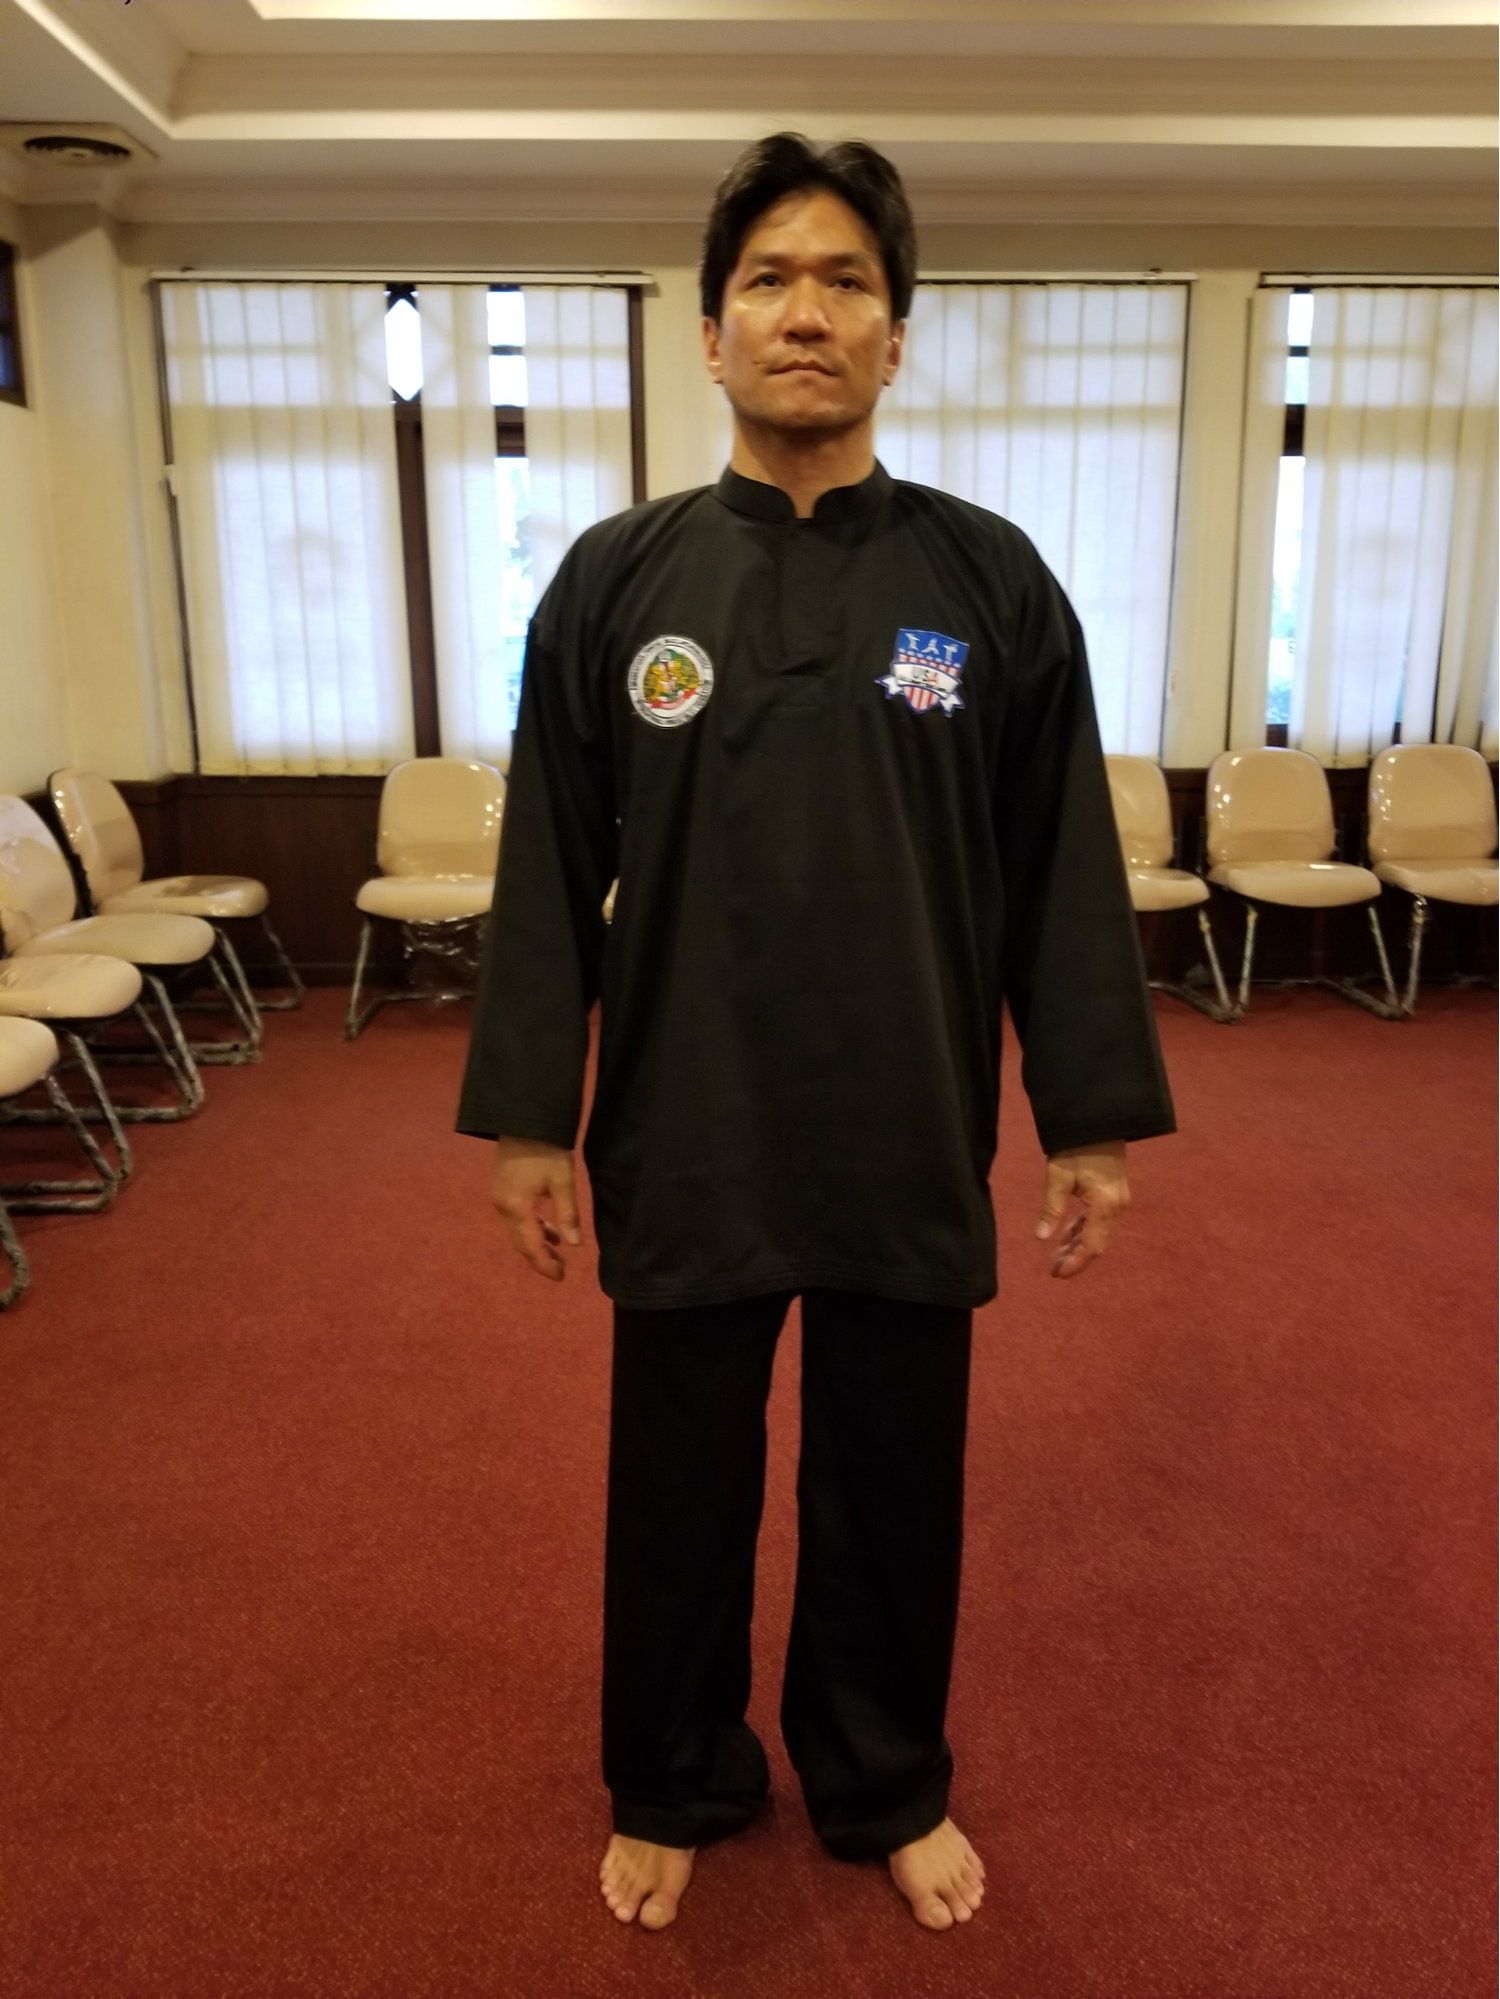
\includegraphics[height=3.0in]{images/tanding_uniform_front}
    }
    ~
    \subfigure[Full Competitor's Tanding Uniform with Sash]{\label{fig:tanding_uniform_pesilat}
        \includegraphics[height=3.0in]{images/tanding_uniform_pesilat}
    }
    \\
    \subfigure[Tanding Uniform Sleeves and Cuff]{\label{fig:tanding_uniform_sleeves}
        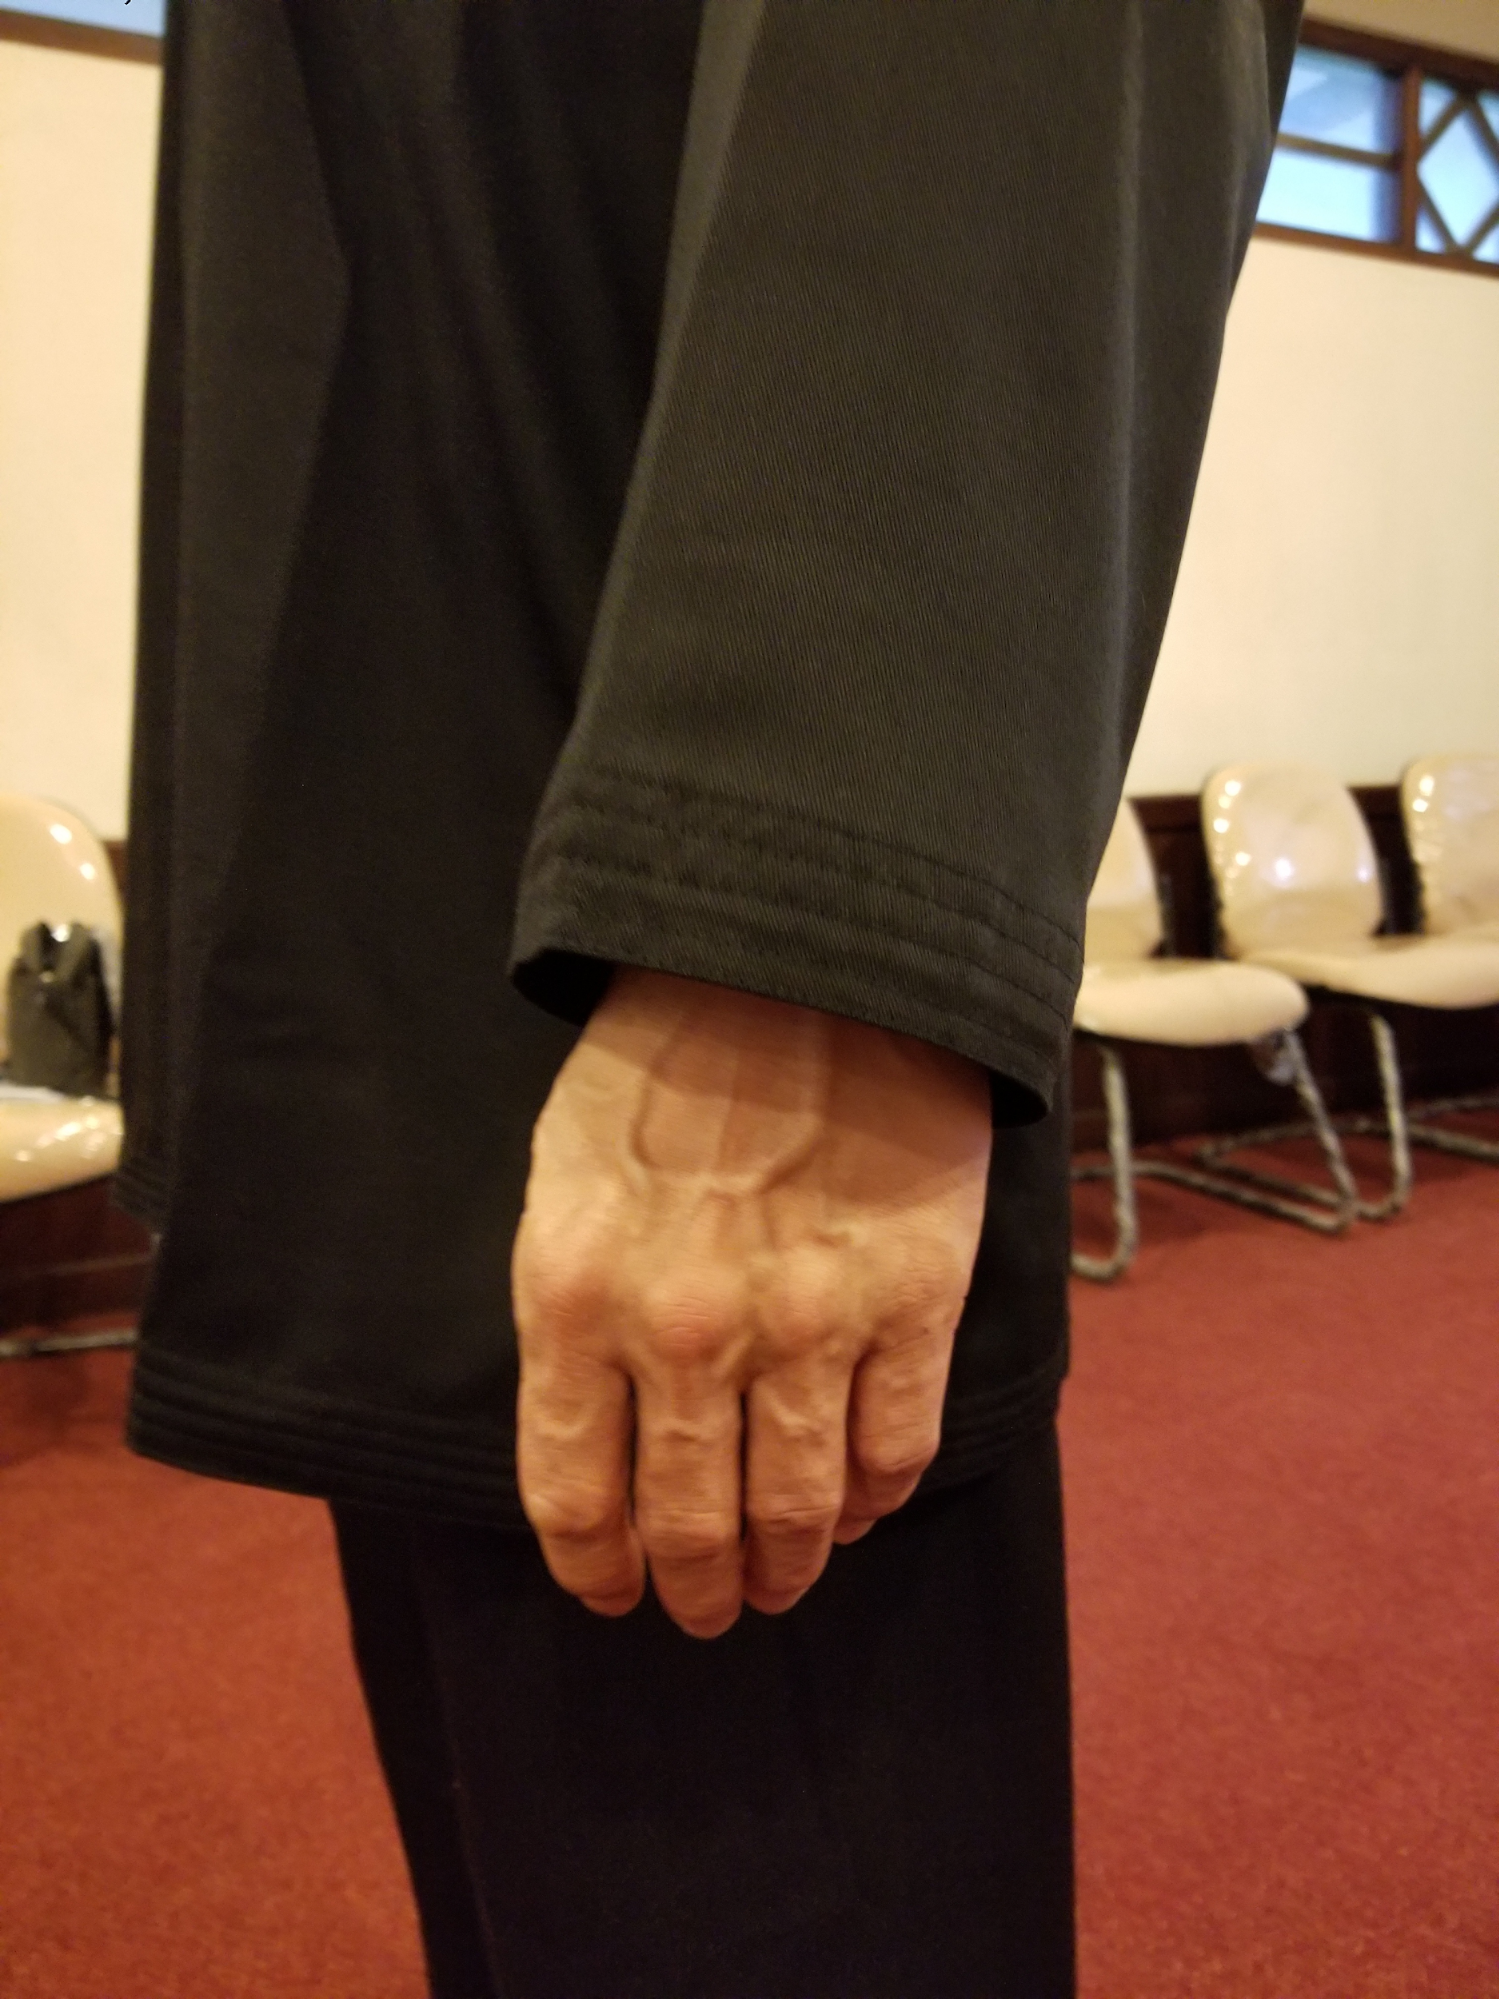
\includegraphics[height=3.0in]{images/tanding_uniform_sleeves}
    }
    ~
    \subfigure[Tanding Uniform Back]{\label{fig:tanding_uniform_back}
        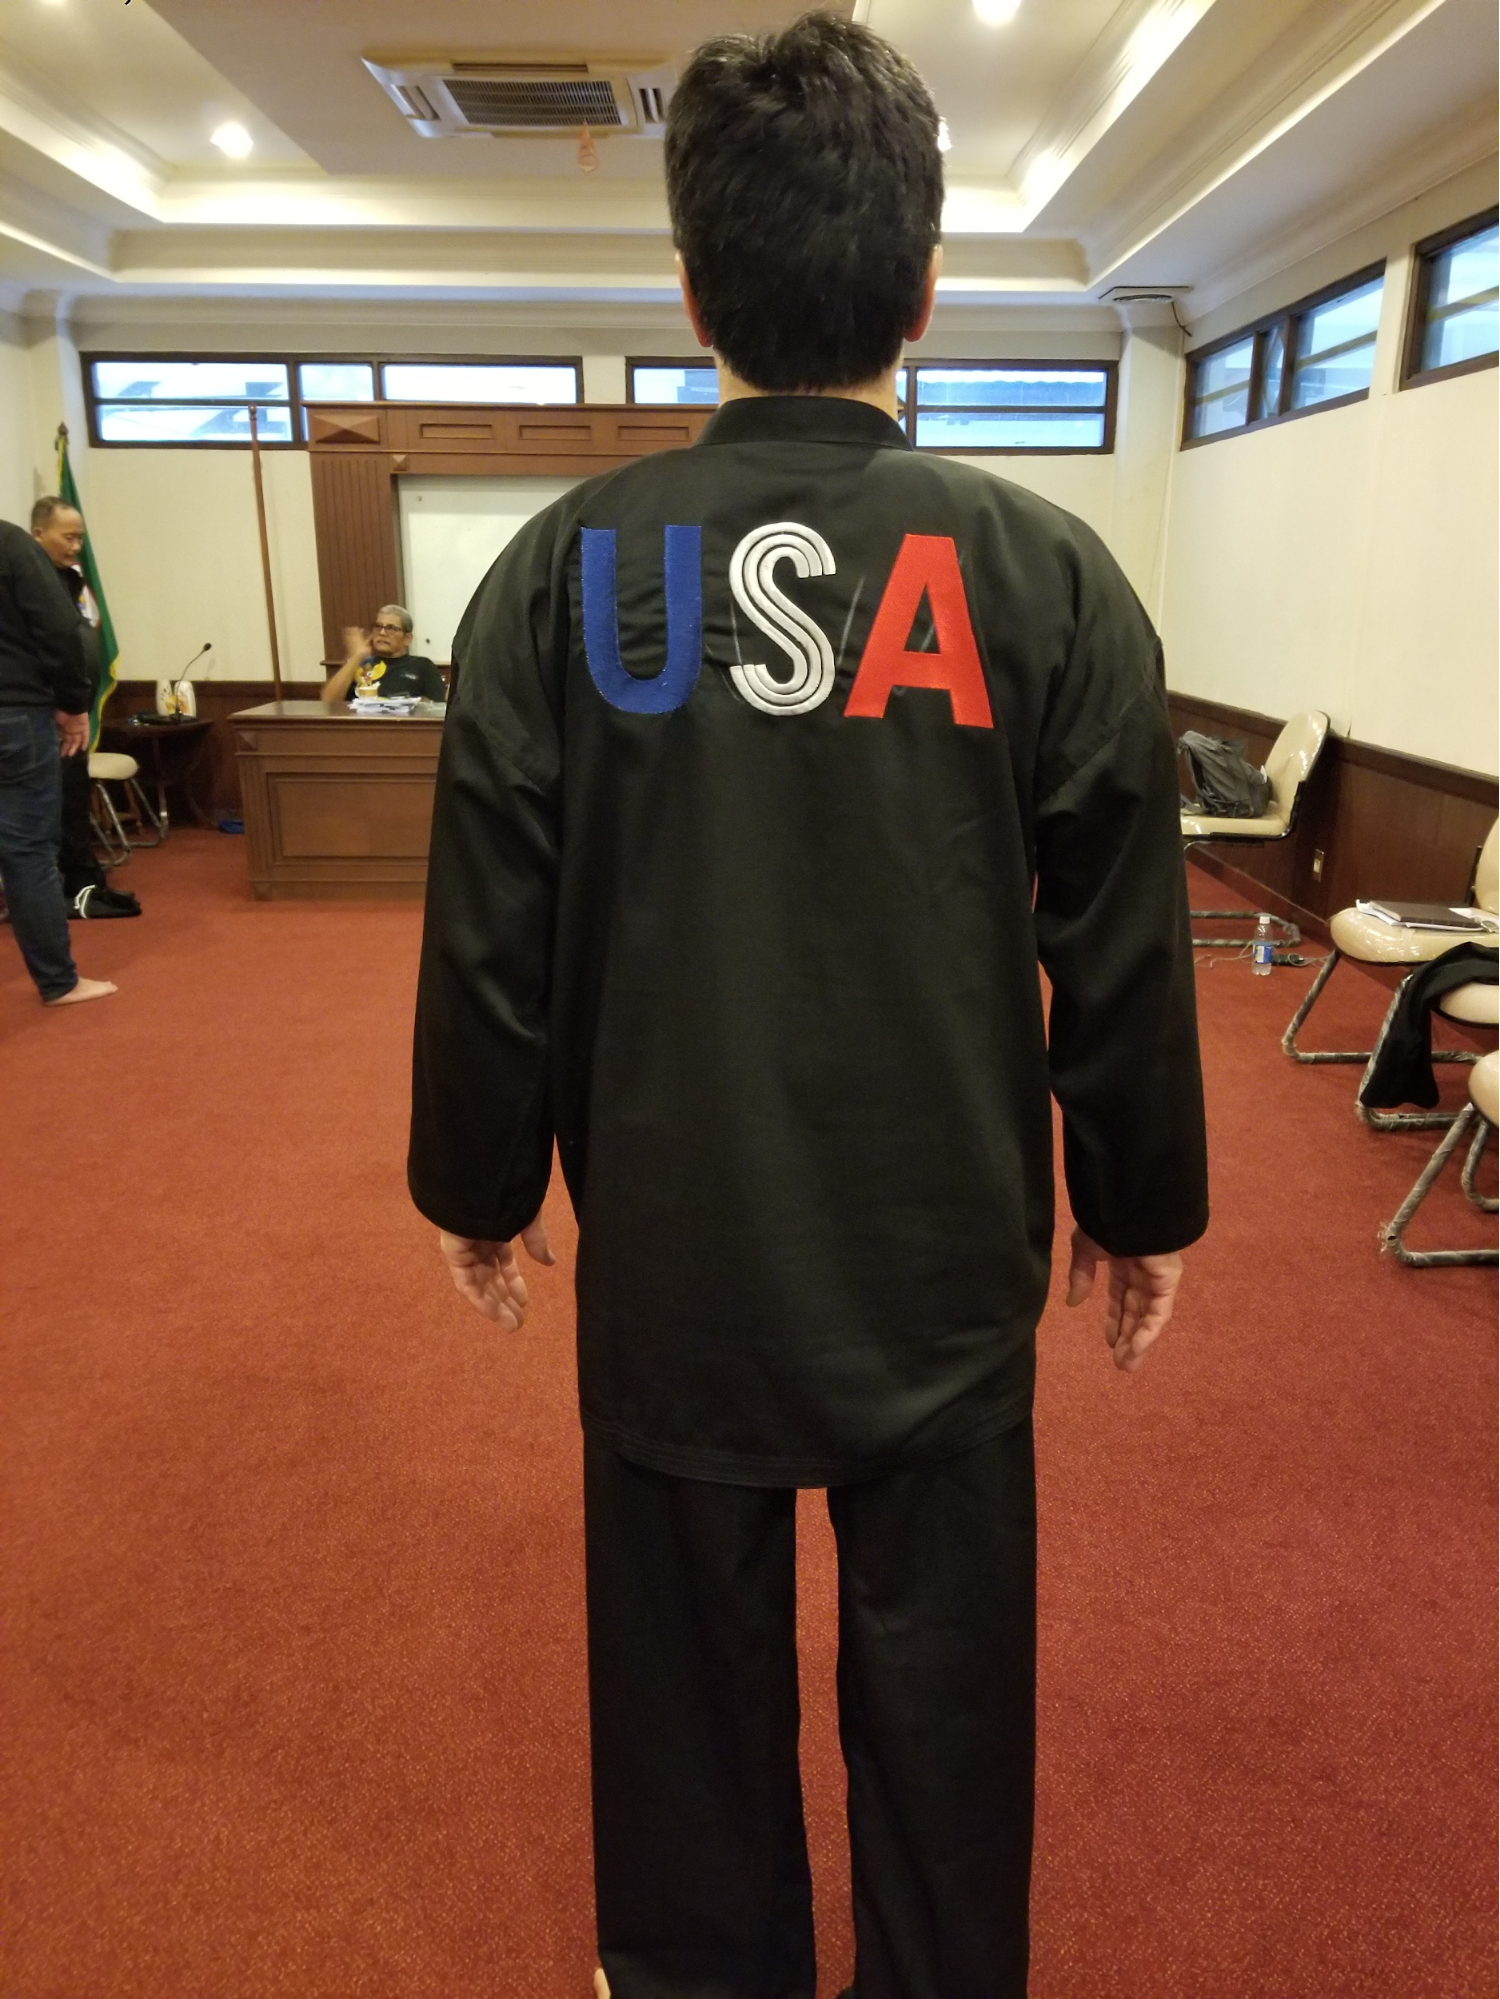
\includegraphics[height=3.0in]{images/tanding_uniform_back}
    }
    \caption{Example Tanding Attire and Details}
    \end{figure}


    \item Body Protector with the following regulations:
    \begin{legal}
        \item PERSILAT quality standard
        \item Black colored
        \item Five sizes: Super Extra Large (XXL), Extra Large (XL), Large (L), Medium (M), and Small (S)
        \item A red or blue sabuk/bengkung (belt/sash) for Pesilat’s corner identification. Size 10cm wide made from uneasy to fold material
        \item One arena should provide at least 5 (five) sets of body protectors of every size that is provided by the Organizing Committee. Mandatory for all athletes to put on the body protectors provided by the Organizing Committee.
    \end{legal}

    \item Groin Protection
    
    It is mandatory for all Male/Female contestants to wear a plastic groin guard provided by the Pesilat (contestant).

    \item Joint Guards

    Joint guards (wrist, ankle, knee, shoulder and elbow), shin and arm guards are allowed to be used in only 1 layer with 1 cm maximum thickness and made from non-hard materials.

    \item Joint Taping is allowed

    \item Mouth guards are allowed
    \end{legal}

\item System and Competition Rounds
    \begin{legal}
    \item Competition uses knock out system. Other systems may be adopted by PERSILAT as and when required.
    \item The competition stages are divided into elimination round, quarter final round, semifinal round and final round, depending on the number of participants. This competition stages shall apply to all classes.
    \item Each competing class should be participated by at least 2 (two) Pesilat (contestants).
    \end{legal}

\item Match Rounds and Time
    \begin{legal}
    \item A match is carried out in 3 (three) rounds. 
    \item Each round takes exactly 2 (two) minutes net. 
    \item Between rounds there is a one-minute net rest.
    \item Moments when the Referee stops the match are not included in the match time. (The counting towards a Pesilat who is knock-downed due to a valid attack is not included in the match time)
    \end{legal}


\item The Pesilat’s Coach
    \begin{legal}
    \item Each Pesilat, particularly in Tanding (Sparring Match) category, is assisted by 2 (two) coaches maximum and understand the Rules and Regulations of Competition of PERSILAT.
    \item The coach’s attire is a PERSILAT standard black Pencak Silat attire (Figure~\ref{fig:tanding_coach}), the sleeves up till
the wrist (+/- 1cm) and the length of the pants up to the ankle (+/- 1cm) with badge
of his/her main association on the left chest and is allowed to put PERSILAT badge on
the right chest, name of the country on the back and wears an orange sash of 10-cm wide.
    \item The coach is allowed to give advice only during rest between rounds.
    \item One of the coaches must be of the same gender with the Pesilat (contestant).

    \begin{figure}[t!]
        \centering
        \subfigure[Coach]{\label{fig:tanding_coach}
            \includegraphics[height=2.5in]{images/tanding_coach}
        }
        ~
        \subfigure[Wasit (Referee) / Judge (Juri)]{\label{fig:tanding_wasit_juri}
            \includegraphics[height=2.5in]{images/wasit_juri}
        }
        ~
        \subfigure[Competition Chairperson]{\label{fig:tanding_chairperson}
            \includegraphics[height=2.5in]{images/chairperson}
        }
        \caption{Competition Officials}
    \end{figure}
    \end{legal}

\item Competition Procedure
    \begin{legal}
    \item The competition is commenced by the Referee and Jury \ref{fig:tanding_wasit_juri} 
    entering the arena from the
    right side of the Competition Chairperson \ref{fig:tanding_chairperson}. 
    Before entering the arena Referee and Jury bow and report to the 
    Competition Chairperson that they are ready to carry out their duties.
    \item Referee shall check the athlete at their individual corners before commencing the
    match. At Referee’s signal, each Pesilat enters the arena from his/her corner,
    bowing/signal respecting to the Coaches, Referee and the Competition Chairman. Afterwards each
    Pesilat is required to perform 5 (five) to 10 (ten) school’s movement (jurus
    perguruan) before returning to their respective corners.
    \item The match will commence by the Referee calling both Pesilats. The Pesilats will then
shake hands, reminding on the rules and be ready for the match.
    \item After the Referee checks the readiness of all officials by means of right hand signal,
he commands both Pesilats to begin the match.
    \item During break time, both Pesilats must return to their respective corners.
    \item Beside the Referee and the two contestants, no one else may enter the arena unless
otherwise, upon the Referee’s request.
    \item At the end of the final round, both Pesilats return to their respective corners to wait
for the decision of the winner. By the time to announce the winner, Referee calls both
Pesilats to the center of arena. Upon announcement of winner, Referee will lift the
winner’s hand. After that both Pesilat respect the Competition Chairman.
    \item After paying respect, both Pesilat’s shake hands and leave the arena. The Referee and
Jury shall come forward in front of the Chairman and give respect, and report to the
Competition Chairman about the completion of their duties. The Referee and Jury
leave the area via the left side of Competition Chairman’s table.
    \end{legal}

\item The Rules of the Game:
    \begin{legal}
    \item The Rules of the Game:
        \begin{legal}
        \item The Pesilats confront each other by applying the Pencak Silat defense and attack
              elements ie. Repulsing, dodging, hitting the target, dropping the opponent; and
              complying to the Pencak Silat Rules and Regulations.
        \item  By applying the `\emph{Pencak Silat principle}', it means to obtain technical scores, a Pesilat
               must apply a combative pattern which consists of on-guard position (sikap-pasang),
               step pattern (pola langkah, Figure~\ref{fig:pola_langkah}), maintain the distance 
               against the opponent, while
               performing the attack/defense, and finally return to the on-guard position (sikap
               pasang, see Figure~\ref{fig:sikap_pasang}).

            \begin{figure}[t!]
                \centering
                \includegraphics[width=4.0in]{images/pola_langkah_dasar}
                \caption{Example Footwork Patterns (Pola Langkah)}
\label{fig:pola_langkah}
            \end{figure}

            \begin{figure}[ht!]
            \centering
            \subfigure[]{\label{fig:sikap_pasang_1}
                \includegraphics[height=1.5in]{images/sikap_pasang_1}
            }
            ~
            \subfigure[]{\label{fig:sikap_pasang_2}
                \includegraphics[height=1.5in]{images/sikap_pasang_2}
            }
            \subfigure[]{\label{fig:sikap_pasang_3}
                \includegraphics[height=1.5in]{images/sikap_pasang_3}
            }
            ~
            \subfigure[]{\label{fig:sikap_pasang_4}
                \includegraphics[height=1.5in]{images/sikap_pasang_4}
            }
            \caption{Example Sikap Pasang}
            \label{fig:sikap_pasang}
            \end{figure}


 
        \item Defense and/or attack must start from on-guard position (sikap pasang),
        followed by a step pattern (pola langkah), with demonstration of good coordination in
        performing an attack defense.  After performing an attack/defense, Pesilat must return on to 
        the on-guard applying step pattern. The Referee will give command `\emph{Langkah}' if a Pesilat 
        does not use proper technique of Pencak Silat.
        \item A series of attacks should be delivered in row, a combination of various
        techniques towards the target, with not more than 6 (six) techniques of attacks, per
        exponent. A Pesilat who performs more than 6 (six) techniques of attacks in a row will
        be stopped by the Referee.  
        Continuous attacks with the hand using the same technique will only score 1 point.
        \item An attack that scores points hits the target by applying the principles and 
        is stable and powerful.
        \end{legal}

        \item Competition Commands
        \begin{legal}
        \item The command `\emph{BERSEDIA}' (Get Ready) is used to alert both Pesilat and 
        all competition officials to be ready as the match is about to begin. The command shall
        be used throughout the match.  Approximate English pronunciation \emph{burr-said-E-ah}.
        \item  The command `\emph{MULAI}' (Start) is used each time a match is started or continued.
This command is used together with the hand signal.  Approximate English pronunciation: \emph{moo-lie}.
        \item The command `\emph{BERHENTI}' (Stop) or `\emph{TI}' is used to stop the match.  Approximate English pronunciation: \emph{burr-hen-tee}.
        \item The commands `\emph{PASANG}', `\emph{LANGKAH}', and `\emph{SILAT}' are used to give guidance.  Approximate English pronunciations: \emph{paw-song}, \emph{long-caw}, \emph{see-lot}.
        \item The start and the end of each round is marked by a strike on the Gong.
        \end{legal}


    \item Targets\\
    A target is defined as the valid areas for attacking for which points can be awarded.  They
    are on the body covering the trunk area excluding the neck and upwards and the navel to the groin.
    Figure~\ref{fig:attacking_targets} illustrates some of the following targets:
        \begin{legal}
        \item Chest
        \item Abdominal (navel upwards)
        \item Left and right ribs
        \item Back part of the trunk (except direct attack to the whole spinal cord)
        \\
    The lower limb (ankle and below) can be targeted for an intercepting attack while aiming to
    drop the opponent but is a non-scoring area.

        \begin{figure}[h!]
            \centering
            \includegraphics[width=4.0in]{images/attacking_targets}
            \caption{Valid Attacking Targets}
            \label{fig:attacking_targets}
        \end{figure}

        \end{legal}
    
    \item Prohibitions \\
    Prohibitions which are declared as violations:
        \begin{legal}
        \item Serious violations
            \begin{enumerate}[label=\alph*.]
            \item Attack illegal parts of body ie. Neck, head and navel downwards to groin,
            direct attack to the whole spinal cord, thigh and lower limbs shin area.
            \item Direct attempts to break the joints.
            \item Deliberately throw the opponent out of the arena
            \item Attack with head (Head Butt)
            \item Attack the opponent before the `\emph{MULAI}' command or after the `\emph{BERHENTI}'
            command is given by the Referee, causing injury to the opponent.
            \item Wrestle, bite, scratch, grip, and pull the opponent’s hair/jilbab (pull hair/jilbab)
            \item A Pesilat challenges, humiliates, hits, utters vulgarities, spits, shouts to
                  provoke opponent or Competition Officials (Technical Delegate,
                  Competition Chairman, Council of Referee-Jury, Referee-Jury and all other
                  officials on duty), and to all spectators.
            \item Slamming down the opponent in or out of arena within the match period.
            \item Gripping, grabbing or embrace while attacking.
            \end{enumerate}

        \item Light violations
            \begin{enumerate}[label=\alph*.]
            \item Does not use on-guard position and step pattern.
            \item Walks out of the arena (any one leg out of the arena) whether intentionally
                  or unintentionally more than 1 (one) time in 1 (one) round
            \item Embrace the opponent in process of defending
            \item Attack with front/back sweeping technique, scissoring while in lying
                  position more than 1 (one) time in 1 (one) round to waste time.
            \item Communicate with outside or coaches either by certain gesture/signals or
by spoken words
            \item Both Pesilats are passive or when one of Pesilat is passive more than 5
seconds.
            \item  Shouting during competing.
            \item Wrong direction of attack.
            \item Intentionally push the opponent out of the arena.
            \item Athlete that turns his/her back against the opponent to waste time or
                  prevent an attack.
            \item Time delaying tactics (releasing the body protector knot, untying of the
hairband, was given the counting etc)
            \end{enumerate}

        \end{legal}

    \item Improper Defense Technique
        \begin{legal}
        \item A valid attack with accurate direction but may cause injury to the opponent 
             due to improper defensive technique (i.e.\ dodging towards the incoming attack)
             direction is not a violation.
        \item If the attacked Pesilat is injured, the Referee will call for the doctor
              immediately. If the doctor decides that the injured Pesilat is unfit to continue fighting,
              the Pesilat will be declared defeated by `technical knock-out' (TKO).
        \item If the doctor declares that the injured Pesilat is fit to continue, but he/she fail
              to stand up at once, the Referee will immediately start the technical counting.
        \end{legal}

    \item Penalties\\
    Level and types of penalties
        \begin{legal}
        \item Reprimand
            \begin{enumerate}[label=\alph*.]
            \item Given when a Pesilat commits light violation after 1 (one) time verbal warning of
                  the same violation within the same round.
            \item Reprimand can directly be given when a Pesilat commits severe violation without
                  causing injury to the opponent.
            \end{enumerate}

        \item Warnings shall be valid for all rounds only for severe violations. 
              For light violation, it ends at every round, consist of:
            \begin{legal}
            \item Warning I \\
            Warning I is given when a Pesilat:
                \begin{enumerate}[label=\alph*.]
                \item Commits severe violation causing injury to opponent
                \item Given third reprimand as the result of light violation
                \end{enumerate}

            After Warning I is given, another reprimand will be given for another type of
            violation within the same round.

            \item Warning II \\
            Warning II is given when a Pesilat commits another severe violation after Warning I.
            Warning II is given, another reprimand will be given for another type of light
            violation within the same round.

            \item Warning III \\
            Warning III is given when a Pesilat commits another severe violation after

            Warning II and will be immediately disqualified.

            Warning III should be shown by the Referee.

            \item Disqualification \\
            Is given when a Pesilat:
                \begin{enumerate}[label=\alph*.]
                \item commits another severe violation after Warning II.
                \item commits serious violation deliberately and contradicts against the
                      sportsmanship.
                \item commits serious violation which receives Warning I or Reprimand
                      I, and the injured opponent is unfit to continue the match as per officiating
                      Doctor’s decision.
                \item fails to meet the weight requirement during the second weigh-in conducted 15
                      minutes before the match.
                \item fails the doping test. A Pesilat that fails the doping test will be
                      disqualified. All medals, certificates and all other awards shall be returned
                      to the Organizing Committee.
                \item is unable to provide the letter of medical checkup before starting the
                      first match (regardless of category) of the competition.
                \end{enumerate}
            \end{legal}


        \end{legal}

        \item Scoring\\

            \begin{legal}
            \item Scoring Rules \\
        \begin{table}[h!]
        \centering
        \begin{tabular}{l|ll}
        Total     & \multicolumn{2}{l}{Breakdown} \\
        \hline
        Score +1  & +1  & An attack by hand/elbow successfully hitting the target without being blocked \\
        \hline
        Score +2  & +1  & Successfully voiding opponent’s attack \\
                  & +1  & AND immediately followed by a successful counter attack by hand. \\
        \hline
        Score +2  & +2  & An attack by foot/knee successfully hitting the target without being blocked. \\
        \hline
        Score +3  & +1  & Successfully voiding opponent’s attack \\
                  & +2  & AND immediately followed by a successful counter attack by foot. \\
        \hline
        Score +3  & +3  & Direct attack that successfully drops the opponent. \\
        \hline
        Score +4  & +1  & Successfully grabbing the opponent's leg \\
                  & +3  & AND immediately followed by a successful dropping technique.\\

        \end{tabular}
        \caption{Technical performance score breakdown}
        \label{tbl:tanding_technical_score}
        \end{table}

            \item Qualifications of Technical Score: (valid scoring) \\
                  Valid score shall be given to the following:
                \begin{enumerate}[label=\Alph*.]
                \item Blocking or evading followed by an immediate valid counter attack
                \item Valid hand attack
                \item Valid foot attack
                \item Valid dropping technique
                \end{enumerate}
                
                \begin{enumerate}[label=\Alph*.]
                \item Blocking or evading -– successfully void the opponent’s attack followed
                      with immediate valid counter attack, either with the foot, hand or
                      dropping attack. \\
                Note: The score of ``1+'' shall be given for successfully voiding the
                      opponent’s attack followed with immediate valid counter attack, either
                      with the foot, hand or dropping attack. Whereby a direct successful
                      attack shall be given points as per its mode: 1 point = hand attack (direct elbow), 
                      2 points = foot attack (knee) and 3 points = valid drop. (no points shall be given
                      for any blocking or evading without counter attack)
                \item Valid hand attack – all types of hand attack which is direct and powerful.
                      (punches from; front, spade, uppercut, side hook and elbow): +1 point
                \item Valid foot attack – all types of foot attack which is direct and powerful.
                      (kicking techniques; frontal, spinning back, side, half-turn, stomping and knee): +2 points
                \item Valid dropping – all applicable techniques to drop the opponent
                      ensuring that the knee and above touches the floor: +3 points
                    \begin{enumerate}[label*=\arabic*.]
                    \item Applying the direct attack such as sweeping, scissors and lifting with the leg.
                    \item Applying indirect dropping technique by catching of opponent’s
                        leg followed by a valid drop (no punching or kicking at this stage).
                    \item Does not drop together with opponent while applying the valid drop technique.
                    \item Dropping process is given duration of 5 seconds before the Referee stops the fight.
                    \item It is not allowed to wrestle before the techniques; sweeping
                        side drop, lifting with the leg or scissors is used. However,
                        pushing or touching is allowed within the body area.
                    \item A counter attack is allowed when a failed sweeping technique
                        occurs. The score for the counter attacks is determined by the
                        technique applied, without using the body weight within one
                        second period.
                    \end{enumerate}
                \item Other factors in the competition
                    \begin{enumerate}[label*=\arabic*.]
                    \item Concurrent attack is an attack (whether valid or invalid, since
                        those attacks happened accidentally) where one or both of
                        Pesilat fall down, the dropping will be validated by the following criteria:
                        \begin{enumerate}[label*=\arabic*.]
                        \item If one of them is not able to get up, counting will be applied immediately.
                        \item If both of them are not able to get up at once, counting will be applied 
                            immediately to both of them.
                        \item If both Pesilats are not able to get up by count of ten (10),
                            however, both had gained points, the winner will be the one
                            with the highest score.
                        \item If the incident occurs during the beginning of the first
                            round and neither of them gains a score, the decision of the
                            winner according to Chapter~\ref{chp:rules_of_the_game} \ref{sec:tanding_category} point~\ref{pt:victory_decision} \ref{pt:tanding_tie_weight} and \ref{pt:tanding_tie_coin} (no rematch).%article 9 point 6.7.4 a.2_iv and v.  (no rematch).
                        \end{enumerate}
                    \end{enumerate}

                \item Accidental Fall – When a Pesilat falls not because of the opponent’s
                    attack, and not able to get up, he will be given the chance to get up
                    within 10 seconds counting. If the Pesilat is not able to continue the
                    fight, will be declared as lost by `TKO'.

                \item Catching
                    \begin{enumerate}[label*=\arabic*.]
                    \item Catching in a process of dropping an opponent is declared failed when:
                        \begin{enumerate}[label*=\arabic*.]
                        \item The dropping process takes more than 5 (five) seconds, or 
                            dragging/wrestling occurs.
                       \item The attacking Pesilat falls down together in the dropping process.
                        \item If during the dropping process, the caught opponent grabs the shoulder of the 
                           Pesilat trying to drop him/her down, and succeed to drop the him/her within 
                            5 (five) seconds before the Referee gives the command `\emph{BERHENTI}' (stop); 
                            the dropping will be declared as valid.
                        \item If the defending Pesilat touches the neck or head or tugging, causing both 
                            Pesilats to fall down, the tugging Pesilat will be given the `\emph{Teguran}' 
                            (reprimand).
                        \end{enumerate}
                    \end{enumerate}

                \item Dropping
                    \begin{enumerate}[label*=\arabic*.]
                    \item When dropping technique is successful, at least part of the body
                       is inside the arena’s boundary line, the dropping will be
                        declared `valid'.
                    \item When a dropping technique is successful within the arena, and
                        the dropped Pesilat shifts out of the arena the dropping will be
                       declared valid.
                    \item  When a valid attack causes the opponent to fall, and unable to get 
                        up immediately, and within the arena, but the dropped Pesilat shifted himself/herself 
                        out of the arena; valid drop signal shall be given immediately. The dropped Pesilat 
                       will be given chance to stand-up and be on-guard position within 10 (ten) seconds, 
                        failing which the dropped Pesilat is unable to continue the bout, he/she will be 
                        declared losing by TKO.
                    \end{enumerate}
                \end{enumerate}

            \item Penalty

            The progression of point deductions for a penalty are:
                \begin{enumerate}[label*=\arabic*.]
                \item Score -1 (minus 1) is given when a Pesilat gets Reprimand I
                \item Score -2 (minus 2) is given when a Pesilat gets Reprimand II
                \item Score -5 (minus 5) is given when a Pesilat gets Warning I
                \item Score -10 (minus 10) is given when a Pesilat gets Warning II
                \end{enumerate}


            \item Victory Decision \label{pt:victory_decision}
                \begin{enumerate}[label=\alph*.]
                \item Win by Points Score
                    \begin{enumerate}[label*=\arabic*.]
                    \item When a majority of the Juries decides in favor of one Pesilat over another
                        than the opponent.
                    \item In the event where there is a tie, the winner will be determined base on the 
                        following:
                        \begin{enumerate}[label=\roman*.]
                        \item With the least penalty scores
                        \item With the most technical scores binned and prioritized as follows: 
                            1+3, 3, 1+2, 2, 1+1, 1
                        \item An additional round
                        \item \label{pt:tanding_tie_weight} The Pesilat who is lighter (body mass) referring to the weight taken at the re-weighing process, 15 minutes before the game.  and witnessed by Technical Delegate and both team managers
                        \item \label{pt:tanding_tie_coin} A coin toss coins to be carried out by the Chairman of Competition and witnessed by Technical Delegate and both team managers
                        \end{enumerate}

                    \item The Jury’s scores shall be displayed on the scoreboard, at the end of the final
                        round, after the winners decision was announced, except if digital scoring system
                        us used (where the scores will be shown in the screen automatically).
                    \end{enumerate}

                \item Win by Technical Knock Out (TKO) of Opponent is declared winning by 
                    Technical Knock Out when:
                    \begin{enumerate}[label=\arabic*.]
                    \item Opponent requests not to continue the fight.
                    \item Competition Doctor’s decision. Competition Doctor is given 120 (One hundred
                        and twenty) seconds to decide whether Pesilat is declared ‘Fit’ or ‘Unfit’ to
                        continue the fight and to give medical help.
                    \item Coach’s request (throw in towel).
                    \item Referee’s decision. (Upon counting of Pesilat to the count of 10).
                    \end{enumerate}

                \item  Win by Absolute Victory\\
                    The decision of absolute victory is made when the opponent is knocked down due to
                    valid attack and he/she is unable to get up immediately and or feels dizzy or unable to
                    stand upright with `sikap pasang' after Referee’s counting up to 10.

                \item Win by RSC (Referee Stop Contest). \\
                    Winning as the referee deems the bout is unbalanced.

                \item Win by WO (Walkover) \\
                    The opponent did not show up in the arena after the third call, with the interval of 30
                    seconds at each call. Unless the Team Manager had informed the withdrawal of the
                    Pesilat.

                \item Win by Disqualification: \\
                    \begin{enumerate}[label=\arabic*.]
                    \item The opponent gets Warning III after Warning II
                    \item The opponent commits a serious violation and is directly punished with disqualification
                    \item The opponent commits a severe violation injuring the opponent hence he/she is not able
                        to continue, and to be decided by the competition’s doctor. A Pesilat who won by
                        disqualification by this rule, will only be allowed to compete in the next match,
                        with the permission and recommendation from competition’s doctor before the
                        next match.
                    \item During weighing, the Pesilat’s weight does not meet the weight requirement.
                    \item Pesilat failed to show the medical certification before the competition started.
                    \end{enumerate}

                \end{enumerate}
            \end{legal}
    \end{legal}
\end{legal}



\newpage
\section{TUNGGAL (Solo Performance) Category}
\label{sec:tunggal_category}


\begin{legal}
\item Competition Equipment:
    \begin{legal}
    \item \strong{Attire:}\\

    A standard Pencak Silat attire (Figure~\ref{fig:tunggal_ganda_attire} of any color and plain (The top and bottom pieces may be of the same or different color). A headband (a veil not covering face, is not consider as a headband) and ‘kain samping’ of plain color or patterned. The color choice and combination are entirely at the discretion of the Contestant. It is allowed to have the badge of the contestant’s main association on the left chest and PERSILAT badge on the right chest. The national flag on the left arm and the name of the country at the upper back of the attire.

    
    \item \strong{Weapons:}\\
    For Senior, golok or parang (Figure~\ref{fig:golok}) is made of metal or wood, non-sharp pointed with length 
    between 30 cm up to 40cm and width of between 2.5 cm to 4 cm.  `Toya' (staff) (Figure~\ref{fig:toya}), 
    is made of rattan with the length of between 150-180 cm and diameter of between 2.5-3.5 cm.

    \begin{figure}[t!]
    \centering
    \subfigure[Tunggal / Ganda Attire]{\label{fig:tunggal_ganda_attire}
        \includegraphics[height=3.0in]{images/tunggal_ganda_attire}
    }
    ~
    \subfigure[Golok / Machete]{\label{fig:golok}
        \includegraphics[height=2.5in]{images/golok}
    }
    ~
    \subfigure[Toya / Staff ]{\label{fig:toya}
        \includegraphics[width=5.0in]{images/toya}
    }
    \caption{Tunggal Weapons}
    \end{figure}

    \end{legal}

\item Competition Stages

    \begin{legal}
    \item When a competition is participated by more than 7 (seven) contestants, a pool system will be implemented.
    \item The three (3) contestants with the highest scores from each pool will compete again in the next round. 
    Unless the following round is the final. The participants of the final round will be the best 3 (three) – in 
    terms of gaining scores – from the previous competition pool stages.
    \item The number of pools is decided in a meeting attended by International Technical Delegates, 
    Competition Chairperson and Council of Jury. The decision will be announced to the participants at the 
    Technical Meeting.
    \item The pool division for contestants is determined by drawing of lots during the Technical Meeting. 
    Voting method, i.e either manually or digitally will be decided through voting at the Technical Meeting.
    \item \underline{Each category should be have a minimum of 2 (two) participants.} When there are only two participants
    competition goes directly to the final round.
    \end{legal}



\item Duration of Competition\\
The performance duration is 3 (three) minutes.

    \begin{figure}[ht!]
    \centering
    \includegraphics[height=4.0in]{images/performance_arena}
    \caption{Performance Arena}
    \label{fig:performance_arena}
    \end{figure}



\item Competition Procedure
    \begin{legal}
    \item The beginning of competition:
        \begin{enumerate}[label=\alph*.]
        \item Juries reporting for duty to the Competition Chairperson from the right side of the Competition Chairperson
        \item Show respect and readiness to perform duty
        \item Taking the allocated seats
        \end{enumerate}

    \item The weapons that were certified by the Competition Chairperson will be placed at the weapon quarantine station as prepared by the organizing committee.\\

Pesilat/coach will be allowed to collect the weapons just before he/she enter the arena (immediately after his/her name was announced).

    \item Pesilat
        \begin{enumerate}[label=\alph*.]
        \item Entering the arena from the left side of the Competition Chairperson
        \item Walk towards the centre of arena
        \item Pesilat is to place the weapon on the weapon stand (no assistance from coach)
        \item Show respect to the Competition Chairperson and turn back to show respect to the Jury
        \end{enumerate}

    \item Competition Chairperson will signal the Jury, time keeper and other competition officials to alert them 
        that duty is about to begin

    \item The showcase
        \begin{enumerate}[label=\alph*.]
        \item Showcase the Opening PERSILAT greeting
        \item The gong will be stricken to mark the beginning of performance time. Contestant to begin the showcase
        \item Bare hand movement
        \item With the Long knife / Golok
        \item With the long stick / Toya (staff)
        \item The gong will be stricken to mark the end of performing time
        \end{enumerate}
    
    \item At the end of the performance
        \begin{enumerate}[label=\alph*.]
        \item Contestant to show respect to the Jury and Competition Chairperson from the center of the arena
        \item To leave the arena by the left side of the Competition Chairperson
        \end{enumerate}

    \item Time Keeping
        \begin{enumerate}[label=\alph*.]
        \item The Competition Chairperson will make sure / take charge of the showcase time.
        \item The time keeper will keep track of the 3 minutes showcase.
        \item Competition Chairperson will announce the actual showcase time. (If digital scoring is used, 
            the time tracking will be as displayed on the screen)
        \end{enumerate}

    \end{legal}

\item Competition Rules

    \begin{legal}
    \item Rules of the game

        \begin{legal}
        \item Contestant showcases the Jurus Tunggal Baku (Solo Compulsory Movement) in three (3) minutes, 
            begin with bare hand followed with weapon movement follow with long knife (golok) followed by the 
            long stick (toya). \\

            A tolerance period of +/-10 seconds is allowed for Pre-teen and Pre-Junior categories while +/-5 
            seconds for the Junior, Senior and Masters categories.\\

            Should the tolerance period go beyond the limit, penalty will be imposed accordingly.
        
        \item Jurus Tunggal Baku is showcased according to the sequential movement, 
            such as the fixed movement sequence, precise techniques with and without weapons, rhythmic movement, 
            firmness and expression.

        \item \label{pt:failed_to_continue} If the contestant failed to continue his/her performance for whatever reason, the  
            Competition Chairperson will declare he/she as being disqualified.

        \item Uttering of voice is allowed.
        \end{legal}

    \item Penalties
        \begin{legal}
        \item \label{pt:tunggal_deductions} Deduction of points will be imposed as such:
            \begin{enumerate}[label=\alph*.]

            \item Mistake in movement sequence and techniques
                \begin{enumerate}[label*=\arabic*.]
                \item Deduction of one (1) point each time
                    \begin{enumerate}[label=\roman*.]
                    \item mistake in movement sequence details
                    \item mistake in movement techniques
                    \item any missing movement (not done)
                    \item should a Pesilat lose grip of the weapon, as long as it does not touches the ground, 
                        a total of 1 point penalty for each wrong and/or additional movement incurred. 
                    \end{enumerate}
                \end{enumerate}

            \item Time factor
                \begin{enumerate}[label*=\arabic*.]
                \item \label{pt:tunggal_deduction_beyond_time} Beyond tolerance period \\
                    Ten (10) to fifteen (15) seconds – deduction of 10 points for Pre-teen and Pre-Junior 
                    categories and five (5) to ten (10) seconds for Junior, Senior and masters categories.\\

                    Should showcase go beyond these tolerance period the showcase will be stopped and 
                    declared disqualified.
                \end{enumerate}


            \item Other factors
                \begin{enumerate}[label*=\arabic*.]
                \item Exceed the arena limit (10m x 10m) – Deduction of 5 points
                \item Drop of weapon – Deduction of 5 points
                \item Attires is not according to prescription – Deduction of 5 points 
                (eg. Extra accessories, head gear or samping fall or)
                \item \label{pt:tunggal_loose_weapon} Weapon came out loose from the handle or breaking of the long stick. 
                Showcase will be stopped and declared disqualified.
                \end{enumerate}
            \end{enumerate}

        \end{legal}

        \item Other Decisions
            \begin{legal}
            \item The Referee Jury Council has the right to request for amendments of the penalties 
            (impose penalty or withdraw penalty) following 3 or more Jury views and decision. Penalty imposed will be denied if it is only be given by 2 or 1 Jury.
            \item When competition is unable to continue due to:
                \begin{enumerate}[label*=\roman*.]
                \item Juries failed to function (fall sick / injured / unconscious)
                \item Non-Technical factors (Electrical breakdown / disturbance / etc)
                \item External factors (something that is beyond human control, natural disaster etc)

                \end{enumerate}

                \begin{enumerate}[label*=\alph*.]
                    \item Competition chairperson will stop the competition with following guidelines:

                    \begin{enumerate}[label*=\arabic*.]
                    \item Contestant involve (unless the last contestant) will be allowed to showcase the performance again right from the beginning (at whichever round he is contesting) with the same Juries, right after the last contestant completing his/her showcase.
                    \item If it is during the last contestant showcase, contestant will be allowed to re-showcase his performance from the beginning, at the latest 10 minutes after the technical problem is solved.
                    \item The Jury that could not carry out their duty is to be replaced.
                    \end{enumerate}
                \end{enumerate}

            \item \label{pt:tunggal_accident} Competition could not proceed due to any accident caused by the contestant (collision with 
                Juries / Jury was hurt due to weapon flung to them, etc) Contestant will be disqualified. 
                Competition Chairperson will replace the injured Jury (after consultation with Technical Delegate) 
                and competition will resume with the next contestant.
            \end{legal}

            \item Walk-over \\
                Participation will be declared as Walk-over should the contestant fail to report to 
                Competition’s Secretary after being call for the 3rd time.\\
                The interval between the call outs will be at thirty (30) seconds each.

            \item Disqualification \\
                \begin{enumerate}[label*=\arabic*.]
                \item Points given to contestant will be withdrawn should it be realized 
                    (at the end of the showcase) that the contestant failed to showcase the whole package or 
                    had perform the package sequence not in proper order.
                \item Putting on totally non-proper attire (not as stipulated) or using a wrong weapon 
                    (eg. Tombak instead of toya)
                \item Pesilat is unable to continue the showcase due to his own fault.
                \item Matters that are stated at point \ref{pt:failed_to_continue}, \ref{pt:tunggal_deductions} (\ref{pt:tunggal_deduction_beyond_time}), \ref{pt:tunggal_deductions} \ref{pt:tunggal_loose_weapon}, and \ref{pt:tunggal_accident}.
                \item Pesilat is unable to show the letter of medical checkup before starting the first match (regardless of category) of the competition.
                \end{enumerate}

    \end{legal}

\item Scoring
    \begin{legal}
    \item Scoring consists of:
        \begin{legal}
        \item Accuracy score includes the following elements:
            \begin{enumerate}[label*=\alph*.]
            \item The accuracy of movement in each Jurus
            \item The accuracy of movement sequence
            \item The accuracy of jurus sequence

            \end{enumerate}

        The score is obtained from the total number of movements in Jurus Tunggal (100 movements) 
        deducted by the penalty points.

        \item Firmness scores include the following elements:
            \begin{enumerate}[label*=\alph*.]
            \item The firmness of movements
            \item The firmness of movement rhythm
            \item The firmness of movement soulfulness
            \item The firmness of power and stamina
            \end{enumerate}

        Score ranges from 50 to 60 points which is the accumulated score of the four firmness elements.
        \end{legal}

    \end{legal}

\item Decision and announcement of the winner
    \begin{legal}
    \item  \label{pt:tunggal_hi_score} The winner is the contestant who gains the highest score for his/her performance from 3 (three) out of 5 (five) jurors with elimination of the highest and the lowest score.
    \item If the scores are equal, the winner will be determined accordingly:
            \begin{enumerate}[label*=\roman*.]
            \item The contestant who gains the total highest Technique points from the 3 (three) jurors as decided in para \ref{pt:tunggal_hi_score}.
            \item The contestant who gains the highest points in firmness, soulfulness and stamina from 3 (three) jurors as decided in para \ref{pt:tunggal_hi_score}.
            \item The contestant whose duration of performance is the closest to precise time of 3 (three) minutes.
            \item The winner is the contestant who gains the least penalty points.
            \item If the result remains the same, the Competition Chairperson will do a coin toss on to the mat witnessed by Technical Delegate, Council of Juror and Team Managers of respective contestant.
            \end{enumerate}

    \item The score of each contestant is announced after the Jury has finished their task in giving score to all contestant of every Jurus Tunggal (Solo Performance) category. Total obtained scores will be shown in scoreboard while announced by Competition Chairperson except when using digital scoreboard where the scores from each Jury and total scores are displayed in the screen instantly.
    \end{legal}

\end{legal}

\newpage
\section{GANDA (Choreographed Pair Performance) Category}
\label{sec:ganda_category}

            \begin{figure}[ht!]
            \centering
            \subfigure[]{\label{fig:ganda1}
                \includegraphics[height=1.5in]{images/ganda1}
            }
            ~
            \subfigure[]{\label{fig:ganda2}
                \includegraphics[height=1.5in]{images/ganda2}
            }
            \caption{Example Ganda Interactions}
            \label{fig:example_ganda}
            \end{figure}



\begin{legal}
\item Competition Equipment:


    \begin{legal}
    \item Attire: \\

    A standard Pencak Silat uniform (Figure~\ref{fig:tunggal_ganda_attire}) of any solid color (The top and bottom pieces may be of the same or different color) with a headband (a veil not covering the face, is not considered a headband) and `kain samping' of plain color or patterned. The color choice and combination are entirely at the discretion of the Contestant. It is allowed to have the badge of the contestant’s main association on the left chest and PERSILAT badge on the right chest. The national flag on the left arm and the name of the country at the upper back of the attire.

    \item Weapons:

        \begin{figure}[ht!]
        \centering
        \subfigure[Golok / Machete]{\label{fig:ganda_golok}
            \includegraphics[height=2.5in]{images/golok}
        }
        ~
        \subfigure[Toya / Staff ]{\label{fig:ganda_toya}
            \includegraphics[height=1.5in]{images/toya}
        }
        \caption{Compulsory Weapons}
        \end{figure}

        \begin{figure}[ht!]
        \centering
        \subfigure[Keris]{\label{fig:ganda_keris}
            \includegraphics[height=2.5in]{images/keris}
        }
        ~
        \subfigure[Pisau / Knife]{\label{fig:ganda_pisau}
            \includegraphics[height=2.5in]{images/pisau}
        }
        \subfigure[Clurit / Sickle]{\label{fig:ganda_clurit}
            \includegraphics[height=2.5in]{images/clurit}
        }
        \subfigure[Trisula]{\label{fig:ganda_trisula}
            \includegraphics[height=2.5in]{images/trisula}
        }
        \caption{Selected Weapons}
        \end{figure}


        \begin{legal}
        \item The types, size and number of weapons to be used are as follows: \\ 
        
            Compulsory weapons: a golok/parang (short knife, Figure~\ref{fig:ganda_golok}) and 
            toya (long stick, Figure~\ref{fig:ganda_toya}) \\

            Selected weapons: It is compulsory to choose either one of these weapons: Keris (Figure~\ref{fig:ganda_keris}), 
            Pisau (knife, Figure~\ref{fig:ganda_pisau}), Clurit (sickle, Figure~\ref{fig:ganda_clurit}) and 
            Trisula (aka Cabang, Tekpi, Sai, Truncheon, Figure~\ref{fig:ganda_trisula}). \\

            The sequence of using compulsory and additional weapon is up to the discretion of the Pesilat.

        \item  For Senior, golok or parang is made of metal or wood, non-sharp pointed with length between 30 cm up 
               to 40 cm. With a width between 2.5 cm to 4 cm. Toya (long stick), made of rattan with the length of 
               between 150-180 cm and diameter of between 2.5-3.5 cm.

        \item For Junior, Senior and Master. (additional weapon)

            \begin{enumerate}[label=\alph*.]
            \item Knife made of metal or wood, non sharp-pointed with size between 15 cm up to 20 cm.
            \item Keris / sickle, sai made of metal or wood, non sharp-pointed with size between 30 cm up to 40 cm.
            \end{enumerate}

        \item The usage of selected weapon may be one or two pieces of a kind. Usage, technique and type of 
              selected weapons is up to the respective Silat Schools.

        \item The showcase is to begin as follows:
            \begin{enumerate}[label=\alph*.]
            \item To begin with bare-hand movement. \\
                  Free to continue:
            \item One Pesilat using weapon while the other bare-handedly, or both Pesilat using weapon.
            \item During performance the weapon moves (transfer) from one Pesilat to the other.
            \item Release or drop weapon in accordance with the performance description.
            \end{enumerate}

        \end{legal}



    \end{legal}
\item Competition Stages
    \begin{legal}
    \item When a competition is participated by more than 7 (seven) contestant, a pool system will be implemented.
    \item Three contestant with the highest scores from each pool will compete again in the next round. Unless the 
          following round is the final. \\
          The participants of the final round will be the best 3 (three) – in terms of gaining scores – from the 
          previous competition pool stages.
    \item The number of pools is decided in a meeting attended by the International Technical Delegates, Competition 
          Chairperson and Council of Jury. The decision will be announced to the participants at the Technical Meeting.
    \item The pool division for contestants are determined by drawing of lots during the Technical Meeting. Voting method, i.e either manually or digitally will be decided through voting at the Technical Meeting.
    \item Each category should be participated by minimum 2 (two) participants and directly goes to final round.
    \end{legal}

\item Duration of Competition \\

      The performance duration is 3 (three) minutes.

\item Competition Procedure
    \begin{legal}
    \item The beginning of competition:
        \begin{enumerate}[label=\alph*.]
        \item Juries reporting for duty to the Competition Chairperson from the right side of the 
              Competition Chairperson
        \item how respect and readiness to perform duty
        \item Taking the allocated seats
        \end{enumerate}

    \item The weapons that were certified by the Competition Chairperson will be placed at the weapon quarantine station as prepared by the organizing committee. Pesilat/coach will be allowed to collect the weapons just before he/she enter the arena (immediately after his/her name was announced).

    \item Pesilat
        \begin{enumerate}[label=\alph*.]
        \item Entering the arena from the left side of the Competition Chairperson
        \item Walk towards the centre of arena
        \item Pesilat is to place the weapon on the mat (no assistance from coach)
        \item Show respect to the Competition Chairperson and turning back to show respect to the Jury committee.
        \end{enumerate}

    \item Competition Chairperson will signal the Juries, time keeper and other Competition official to alert them that duty is about to begin.

    \item The showcase
        \begin{enumerate}[label=\alph*.]
        \item Showcase the Opening PERSILAT greeting
        \item The gong will be stricken to mark the beginning of performance time
        \item Pesilat will perform the showcase
        \item The gong will be stricken to mark the end of performing time
        \end{enumerate}

    \item At the end of the performance
        \begin{enumerate}[label=\alph*.]
        \item Contestant to show respect to the Juries and Competition Chairperson from the center of the arena
        \item To leave the arena by the left side of the Competition Chairperson
        \end{enumerate}

    \item Time Keeping
        \begin{enumerate}[label=\alph*.]
        \item The Competition Chairperson will make sure/take charge of the showcase time
        \item The Time Keeper will keep track of the 3 minutes showcase
        \item Competition Chairperson will announce the actual showcase time. (If digital scoring is used, 
              the time tracking will be as displayed on the screen)
        \end{enumerate}

    \end{legal}


\item Competition Rules
    \begin{legal}
    \item Rules of the game
        \begin{legal}
        \item For 3 (three) minutes the participant performs the richness technique of jurus attack-defense with bare hands and with weapons.\\
        A tolerance period of +/-5 seconds is allowed.\\
        Should the tolerance period go beyond the limit, penalty will be imposed accordingly.
        \item Uttering of sound is allowed
        \end{legal}

    \item Penalties
        \begin{legal}
        \item\label{pt:ganda_deductions} Deduction of score is imposed each time contestant performs the following faulty:
            \begin{enumerate}[label=\alph*.]
            \item\label{pt:ganda_time_factor} Time Factor
                \begin{enumerate}[label*=\arabic*.]
                \item Beyond the tolerance period
                    \begin{enumerate}[label*=\arabic*.]
                    \item five (5) to ten (10) seconds deduction. Should the showcase go beyond these tolerance 
                    period the showcase will be stopped and declared disqualified.
                    \end{enumerate}
                \item Other factors \\
                    Deduction of 5 (five) points penalty will be imposed to the following:

                    \begin{enumerate}[label=\roman*.]
                    \item Contestant crosses the arena borderline (10m x 10m)
                    \item Each time the weapon drop against prescription
                    \item Weapon did not drop as prescribe in the prescription
                    \item The weapons that was prescribe as drop (in the prescription), drop outside
                        the arena and pesilat crosses the arena to pick the weapon (as it is still needed
                        for the showcase)
                    \item using not fully proper weapon according to the regulation, or broken golok,
                        broken toya, golok loose from its head.
                    \end{enumerate}
                
                \end{enumerate}
            No deduction of score for accessories falls.
            \end{enumerate}
        \item Walk-Out \\
        Participation will be declared as Walk-out should the contestant fail to report to the Competition’s 
        Secretary after being call for the 3rd time.\\

        The interval between the call outs will be at thirty (30) seconds each.

        \item Disqualification
            A Pesilt will be disqualified for:
            \begin{enumerate}[label=\alph*.]
            \item Wearing a non-compliant uniform 
            \item Using a weapon not allowed by competition regulations 
            \item Violating time limits as stated in point~\ref{pt:ganda_deductions}~\ref{pt:ganda_time_factor}.
            \item Being unable to show the letter of medical health before the start of competition 
            \end{enumerate}

        \end{legal}

    \end{legal}

\item Scoring
    \begin{legal}
    \item Scoring consist of:
        \begin{legal}
        \item Score of attack-defense technique:\\
            The score of attack-defense technique – bare-handed or armed, includes various attack-defense 
            techniques by hands or foot such as: hitting, kicking, sweeping, dropping, parrying, 
            dodging/evading, catching, locking, etc.

        Scoring shall focus on the following elements:

        \begin{enumerate}[label=\alph*.]
        \item The quality of attack-defense techniques in barehanded as well as using weapon.
        \item The richness of attack-defense techniques in barehanded as well as using weapon.
        \item The skill and creativity of attack-defense techniques
        \item The logic in executing attack-defense technique
        \end{enumerate}

        Score ranges from 60 (sixty) to 80 (eighty) points which is the total score of the above four elements of technique.

        \item Firmness Score: \\
        Firmness score consists of elements of firmness, harmony, courage of both Pesilats during performance.

        Scoring shall focus on the following elements:

            \begin{enumerate}[label=\alph*.]
            \item Firmness and strictness of movement
            \item Harmony/solidity of both Pesilats
            \item Courage in weapon skill
            \item Power and stamina
            \end{enumerate}

        Score ranges from 50 to 60 points which is the integrated score of the above four elements of firmness.

        \item Soulfulness score includes the following elements:
            \begin{enumerate}[label=\alph*.]
            \item The harmony of expression of movement soulfulness
            \item The harmony of movement rhythm score ranges from 50 (fifty) to 60 (sixty)
                  points which is the integrated score of both elements of soulfulness. 
            \end{enumerate}
        \end{legal}
    \end{legal}

\item Decision and announcement of the winner
    \begin{legal}
    \item\label{pt:ganda_winner} The winner is the contestant who gains the highest score for his/her performance from 3 (three) out of 5 (five) jurors with elimination of the highest and the lowest score.
    \item If the scores are equal, the winner will be determine accordingly:
            \begin{enumerate}[label=\alph*.]
            \item The contestant who gains the total highest Technique points from the 3 (three) jurors as decided in para~\ref{pt:ganda_winner}
            \item The contestant who gains the highest points in firmness, soulfulness and stamina from 3 (three) jurors as decided in para~\ref{pt:ganda_winner}
            \item  The contestant whose duration of performance is the closest to precise time of 3 (three) minutes.
            \item  The winner is the contestant who gains the least penalty points.
            \item If the result remains the same,the Competition Chairperson will do a coin toss on to the mat 
            witnessed by Technical Delegate, Council of Juror and Team Managers of respective contestant. 
            \end{enumerate}
    \item The score of each contestant is announced after the Jury has finished their task in giving score to all contestant of the category.\\

    Total scores will be shown on the scoreboard while announced by the Competition Chairperson except when using a digital scoreboard where the scores from each Jury and total scores are displayed in the screen instantly.

    \end{legal}

\end{legal}

\newpage
\section{REGU (Synchronized Team Performance) Category}
\label{sec:regu_category}

\begin{legal}
\item Competition Equipment:
    \begin{legal}
    \item Attire: \\
        A standard black Pencak Silat attire, with a white belt of 10cm which is wrapped not tied nor loosely, and without accessories. \\

        It is compulsory to have the badge of the contestant’s main association on the left chest and the badge of PERSILAT in the right chest. \\

        It is allowed to have the badge of the contestant’s main association on the left chest and PERSILAT badge on the right chest. The national flag on the left arm and the name of the country at the upper back of the attire.
    \end{legal}

\item Competition Stages

    \begin{legal}
        \item When a competition has more than 7 (seven) contestants, a pool system will be implemented.
        \item The three (3) Contestants with the highest scores from each pool will compete again in the next round. Unless the following round is the final.  The participants of the final round will be the best three (3) – in terms of gaining scores – from the previous competition pool stages.
        \item The number of pools is decided in a meeting attended by International Technical Delegates, Competition Chairperson and Council of Jury. The decision will be announced to the participants at the Technical Meeting.
        \item The pool division for contestants are determined by drawing of lots during the Technical Meeting. Voting method, i.e either manually or digitally will be decided through voting at the Technical Meeting.
        \item Each category should have a minimum of 2 (two) teams. When there are only two teams, the competition goes directly to the final round.
        \end{legal}

\item Duration of Competition \\

      The performance duration is 3 (three) minutes.

\item Competition Procedure
    \begin{legal}
    \item The beginning of competition:
        \begin{enumerate}[label=\alph*.]
        \item Juries reporting for duty to the Competition Chairperson from the right side of the 
              Competition Chairperson
        \item how respect and readiness to perform duty
        \item Taking the allocated seats
        \end{enumerate}

    \item Pesilat
        \begin{enumerate}[label=\alph*.]
        \item Entering the arena from the left side of the Competition Chairperson
        \item Walk towards the centre of arena
        \item Pesilat is to place the weapon on the mat (no assistance from coach)
        \item Show respect to the Competition Chairperson and turning back to show respect to the Jury committee.
        \end{enumerate}

    \item Competition Chairperson will signal the Juries, time keeper and other Competition official to alert them that duty is about to begin.

    \item The showcase
        \begin{enumerate}[label=\alph*.]
        \item Showcase the Opening PERSILAT greeting
        \item The gong will be stricken to mark the beginning of performance time
        \item Pesilat will perform the showcase
        \item The gong will be stricken to mark the end of performing time
        \end{enumerate}

    \item At the end of the performance
        \begin{enumerate}[label=\alph*.]
        \item Contestant to show respect to the Juries and Competition Chairperson from the center of the arena
        \item To leave the arena by the left side of the Competition Chairperson
        \end{enumerate}

    \item Time Keeping
        \begin{enumerate}[label=\alph*.]
        \item The Competition Chairperson will make sure/take charge of the showcase time
        \item The Time Keeper will keep track of the 3 minutes showcase
        \item Competition Chairperson will announce the actual showcase time. (If digital scoring is used, 
              the time tracking will be as displayed on the screen)
        \end{enumerate}

    \end{legal} % 1.1

\item Competition Rules
    \begin{legal}
    \item Rules of the game
        \begin{legal}
        \item The participants perform Jurus Wajib Regu for 3 (three) minutes. 
            A tolerance period of +/- 5 seconds is allowed.  Should the tolerance period go beyond the limit, 
            penalty will be imposed accordingly.
        \item Jurus Wajib Regu is performed according to a fixed sequence of movements and the accuracy of jurus, 
            rhythm, firmness and soulfulness designated for the jurus.
        \item Uttering of sound is allowed
        \end{legal}

    \item Penalties
        \begin{legal}
        \item \label{pt:regu_deductions} The score deduction penalty imposed due to contestants’ fault consists of:
            \begin{enumerate}[label=\alph*.]
            \item Errors in the movement and movement detail
                \begin{enumerate}[label*=\arabic*.]
                \item Deduction of 1 (one) point penalty is imposed each time contestant performs faulty movement i.e.:
                    \begin{enumerate}[label=\roman*.]
                    \item Errors in the movement details
                    \item Errors in movement sequence
                    \end{enumerate}
                \item Every mission movement (not performed)
                \item Each time a movement is not performed in `team-harmony'
                \end{enumerate}

            \item Time factor
                \begin{enumerate}[label*=\arabic*.]
                \item \label{pt:regu_time_factor} Beyond tolerance period \\
                    Ten (10) to fifteen (15) seconds – deduction of 10 points for Pre-teen and Pre-Junior 
                    categories and five (5) to ten (10) seconds for Junior, Senior and masters categories.\\

                    Should showcase go beyond these tolerance period the showcase will be stopped and 
                    declared disqualified.
                \end{enumerate}


            \item Other factors
                \begin{enumerate}[label*=\arabic*.]
                \item Deduction of 5 (five) points penalty will be imposed to the contestant each time they cross 
                    the arena borderline (10m x 10m). – To step out of the arena with even only one foot.
                \item Deduction of 5 (five) points penalty will be imposed to the contestant not properly dressed 
                    according to the rules.
                \end{enumerate}
            \end{enumerate}

        \item Walk-Out \\
            Participation will be declared as Walk-out should the contestant fail to report to the Competition’s 
            Secretary after being call for the 3rd time.\\

            The interval between the call outs will be at thirty (30) seconds each.

        \item Disqualification
            A Pesilat will be disqualified for:
            \begin{enumerate}[label=\alph*.]
            \item Wearing a non-compliant uniform 
            \item Time limit violations as stated in point~\ref{pt:regu_deductions}~\ref{pt:regu_time_factor}
            \item Being unable to show the letter of medical health before the start of competition
            \end{enumerate}
        \end{legal} % 1
    \end{legal} % 1

\item Scoring
    \begin{legal}
    \item Scoring consists of:
        \begin{legal}
        \item Accuracy score includes the following elements:
            \begin{enumerate}[label*=\alph*.]
            \item The accuracy of movement in each Jurus
            \item The accuracy of movement sequence
            \item The accuracy of jurus sequence
            \end{enumerate}
            Score obtained from the total number of movements in Jurus Wajib Regu (100 movements) deducted by the penalty points

        \item The score of harmony, firmness and solidity includes the following elements:
            \begin{enumerate}[label*=\alph*.]
            \item The harmony, firmness and solidity of movement
            \item Rhythm harmony of movement
            \item Soulfulness harmony of movement
            \item Power and stamina
            \end{enumerate}
        Score ranges from 50 (fifty) to 60 (sixty) points which is the total score of the above four elements.
        \end{legal} % 1.1.1
    \end{legal} % 1.1

\item Decision and announcement of the winner
    \begin{legal}
    \item  \label{pt:regu_hi_score} The winner is the contestant who gains the highest score for his/her performance from 3 (three) out of 5 (five) jurors with elimination of the highest and the lowest score.
    \item If the scores are equal, the winner will be determined accordingly:
            \begin{enumerate}[label*=\roman*.]
            \item The contestant who gains the total highest Technique points from the 3 (three) jurors as decided in para \ref{pt:regu_hi_score}.
            \item The contestant who gains the highest points in firmness, soulfulness and stamina from 3 (three) jurors as decided in para \ref{pt:regu_hi_score}.
            \item ) The contestant whose duration of performance is the closest to precise time of 3 (three) minutes.
            \item The winner is the contestant who gains the least penalty points.
            \item If the result remains the same, the Competition Chairperson will do a coin toss on to the mat witnessed by Technical Delegate, Council of Juror and Team Managers of respective contestant.
            \end{enumerate}

    \item The score of each contestant is announced after the Jury has finished their task in giving score to all contestant of every Jurus Regu Wajib (Team) category. Total obtained scores will be shown in scoreboard while announced by Competition Chairperson except when using digital scoreboard where the scores from each Jury and total scores are displayed in the screen instantly.
    \end{legal}
\end{legal} % 1


\newpage
\section{Protest Procedure}\label{sec:protest_procedure}

For all competition categories, procedure of protest shall be governed by the following rules:
\begin{legal}
\item  The Team Manager must file a protest by filling in a form provided by Competition Secretary\\

A request for the `protest form' for all categories must be made within 10 minutes after result of the competition has been announced; and within the following 20 minutes, the completed form must be returned to the Competition Secretary including the protest fee of USD200.00 in cash.

\item In filing a protest, objections must be clearly described.\\

At the first level, the protest will be handled by the Competition Chairperson together with the Council of Referee-Jury. The decision will be conveyed to the Team Manager within 2 (two) hours after the protest is submitted.

\item  If the decision made at first level is not accepted, the Team Mananager may make an appeal. The appeal should be made within 20 minutes after the first-level decision is received.

\item The Appeal Committee shall consists of the International Technical Delegate as the Chairperson, and Competition Chairperson and Council of Referee-Jury Council as members. They will review the case and make decision within 3 (three) hours after the appeal is received. At this level, the decision is final.

\item A protest may be reviewed only if it is submitted properly according to the noble values and ethics of Pencak Silat.

\item  Every protest will be imposed with USD 200 fee, unless USSSA/PERSILAT stipulates otherwise. The protest fee is given to Competition Chairperson through Competition Secretary and will be used for Competition Officials (International Technical Delegate, Competition Chairperson, Council of Referee-Jury and Referee-Jury).
\end{legal}

\section{Technical Meeting}
\label{sec:technical_meeting}

\begin{legal}
\item Technical Meeting must be held before the start of the competition.
\item The meeting is presided by Competition Chairperson accompanied by the ITD and/or
ATD, the Council of Referee-Jury and the Chairperson/representative of the Organizing
Committee.
\item Attended by Team Managers and/or Team Coaches.
\item The meeting agenda is a general explanation on competition matters and balloting
process.
\item If necessary, the Competition Committee may conduct a consultative meeting with
the Team Managers at any time during the championship.
\end{legal}


\chapter{Competition Committee}\label{chp:competition_committee}

\section{Structure and Appointment of Competition Committee}\label{sec:structure_and_appointment_competition_committee}

\begin{legal}
\item Competition Committee consists of:
    \begin{legal}
    \item International Technical Delegate (ITD)
    \item Assistant Technical Delegate (ATD)
    \item Competition Chairperson \\
    To perform his duty, a Competition Chairperson may be assisted by:
        \begin{legal}
        \item Referee Jury Council
        \item Referee Jury Council
        \item Competition Secretary
        \item Time Keeper who also acts as Gong striker and Signal giver.
        \item Arena Assistants as required.
        \item Weigh-in Official
        \end{legal}
    \item Council of Referee-Jury consisting of a Chairperson and 2 members.\\
        To perform the duty is assisted by a number of Referee-Jury. 
        (A total of 15 Referee-Jury is required per arena.)
    \item IT Team (if digital scoring system is used). Maximum 2 people per arena.
    \item Competition Doctor and Medical Team.
    \end{legal}
    If more than one arena is needed, the number of competition officials may be 
    modified accordingly, except the ITD and ATD.
\item Appointment of Competition Committee: \\
For Regional and International championships, the appointment of Technical
Delegate, Assistant Technical Delegate, Competition Chairperson, Council of Referee-
Jury and Referee-Jury should be given by USSSA/PERSILAT upon agreement from individual
states/regions/countries depending on the breadth and level of competition.

\end{legal}

\section{Criteria, Duties and Responsibilities of Competition Committee}\label{sec:criteria_duties_responsibilities_competition_committee}

\begin{legal}
\item The International Technical Delegate (ITD)
    \begin{legal}
    \item The International Technical Delegate (ITD) for international championship is appointed by 
        USSSA/PERSILAT \\
    An ITD must have mastered all PERSILAT General Rules and Regulations, particularly
    the Rules and Regulations of International Pencak Silat Competition.
    \item The Organizing Committee of the competition is fully responsible to ensure the
        presence of the ITD at the competition by facilitating return air tickets,
        appropriate lodging, local transportation, pocket money etc; unless USSSA/PERSILAT
        stipulate otherwise.
    \item Duties and Responsibilities
        \begin{legal}
        \item To assist and to provide advice to the Organizing Committee, and
particularly to the Competition Committee, from preparation stage i.e.
supervising any preparation made by the Organizing Committee such as
equipment and facilities, etc, during the course of competition, and until
the end of the championship.
        \item To resolve any problems concerning general issues as well as technical
matters, of which decision of the ITD has binding force
The right including to stop, postpone, cancel championship and or replace the
Competition Committee if deemed necessary.

Those actions should be taken to secure the championships, technical execution
of championships, and the shake of good image of Pencak Silat.

        \item To fill in and to sign the Record Book of Referee and Jury.
        \item To submit duty report to the Board of PERSILAT within 1 (one) month
after the championship ends.

        \end{legal}
    \end{legal}

\item Assistant Technical Delegate (ATD)
    \begin{legal}
    \item The duty of Assistant Technical Delegate is to assist the ITD.
    \item The ATD who comes from the Organizing Committee of the competition is
appointed by PERSILAT based on the criteria of mastering and comprehending
PERSILAT general rules and regulations and particularly regulations of
international Pencak Silat competitions.
    \item If from the Organizer’s side such person is not available, PERSILAT will appoint ATD.
    \item In performing his duty, the ATD is responsible to the ITD.
    \end{legal}

\item  Competition Chairperson
    \begin{legal}
    \item The Competition Chairperson should be International Referee-Jury of Senior Level 
        (Grade 1 or Grade 2).
    \item Duties and responsibilities:
        \begin{legal}
        \item To manage and to be responsible for the smooth running of the competition.
        \item To chair a technical meeting with all team managers before the start of
competition accompanied by the ITD (International Technical Delegate)
and/or ATD, Chairperson of the Council of Referee-Jury, and Chairperson of
the Organizing Committee.
        \item To warn and if necessary, to replace any technical official after consulting
the ITD, if the pertinent person does not properly carry out his duty and
responsibility.
        \item To stop the course of a contest, if necessary.
        \item To expel the coach of Pesilat if he/she disturb the competition.
        \item To resolve any competition problem at first level after consulting the Council of Referee-Jury.
        \item To forward competition problems to the ITD.
        \item To signal Jury in Tunggal, Ganda and Regu categories when contestant is
        shifting outside the arena borderline (10m x 10m) in front of Competition
        Chairperson.
        \item The Chairperson of Competition is responsible to the ITD.
        \item Competition Chairperson is responsible to the performance time of Tunggal Ganda Regu categories.
        \end{legal}
    \end{legal}

\item Competition Secretary
    \begin{legal}
    \item The Competition Secretary is someone with experience and knowledgeable in
administration of competition and is appointed by the Organizing Committee.
    \item His task is to assist the Competition Chairperson in managing any competition
administrative matters. In carrying out his duties, he may also be assisted by a
Secretary Assistant.
    \item The Competition Secretary is responsible to the Competition Chairperson whereas
the Secretary Assistant is responsible to the Competition Secretary.
    \end{legal}

\item Council of Referee-Jury
    \begin{legal}
    \item The Council of Referee-Jury is the leader of Referee, appointed and assigned by
        USSSA/PERSILAT. The Council consists of a Chairperson and 2 (two) Members.

    \item The authority and responsibility of Council of Referee-Jury is:
        \begin{legal}
        \item To assist the Competition Chairperson in arranging the assignment of Referee-Jury.
        \item To review the Jury’s scoring results and when needed, has the right to call the Jury via the Competition Chairperson.
        \item After the review, to approve the Jury’s scoring results, sign and submit the results to the Competition Chairperson.
        \item To give consideration when a contestant protests the competition result.
        \item The Council of Referee-Jury is technically responsible to the ITD (International
Technical Delegate), and administratively responsible to Organizing Committee.
        \end{legal}
    \end{legal}

\item The Referee and Jury
    \begin{legal}
    \item The assignment of Referee and Jury:
        \begin{legal}
        \item Referee and Jury who will be in charge of a Pencak Silat competition of international level are appointed and assigned by PERSILAT.
        \item The Referee and Jury who will be in charge of a competition should have
attended the course for International Referee-Jury, obtained PERSILAT
Certificates for the International Referee-Jury and eligible for the tasks.
        \item The assignment of Referee and Jury is made by PERSILAT based on their
performance record and License Book.
        \item Each Referee and Jury must be competent to judge in all categories of Pencak Silat 
            competition.
        \end{legal}
    \item At an international competition, the maximum number of Referees and Jury is 15
        (fifteen) persons for one arena and 2 Competition Chairperson and 2 Council
        Referee-Jury.
        \begin{legal}
        \item Competition of Tanding category is conducted by 1 (one) Referee and scored by 5 (five) Jurors.
        \item Competition of Tunggal, Ganda and Regu category is scored by 5 (five) Jurors. The highest score and the lowest score given by 2 (two) Jurors is not counted or deleted. Sum up score given by 3 (three) remaining Jurors is the final score of the contestant.
        \end{legal}

    \item The tasks of Referee (for Tanding category only):
        \begin{legal}
        \item To inspect the readiness of arena and contestants
        \item To direct a contest in compliance with the competition stipulated rules.
        \item To ensure the safety of the contestants.
        \item To stop the contest when:
            \begin{enumerate}[label=\alph*.]
            \item The contestant commits a violation
            \item To contestant shifts outside of the arena
            \item The contestant falls down
            \item The contestants wrestle
            \item The match is unbalanced
            \item Issuing Reprimand (Teguran), Warning (Peringatan) or Penalty (Hukuman)
            \item Examining contestant’s wounds/injury
            \item The course of the contest is disturbed
            \item The contestant withdraws from the competition
            \item Requested by the Competition Chairperson or the International Technical Delegate (ITD)
            \item Etc.
            \end{enumerate}
        \item To maintain the quality of the contest
        \item To give the reprimand, warning and penalty to Pesilat
        \item To give signal to the Jury on violation and penalty imposed to a Pesilat, and on the validity of a dropping attack.
        \item To consult the Jury when any doubt occurs in decision-making. The Jury will be called by Referee to ask for decision in the centre of the arena witnessed by one Council of Referee-Jury, after the Pesilats are sent to the neutral corners
        \item To execute winning decision
        \end{legal}
    \item The tasks of Jury (for all competition categories):
        \begin{legal}
            \item To record violations
            \item To decide the winner based on score
            \item To decide the winner based on score
            \item To answer any question which may come from ITD, Competition Chairperson, Council of Referee-Jury or Referee.
        \end{legal}

    \item On duty, the Referee-Jury is technically responsible to the Council of Referee-Jury,
and subsequently also responsible to the Competition Chairperson and finally
responsible to the ITD appointed by PERSILAT.
    \end{legal}
\item Time Keeper
    \begin{legal}
    \item The Time Keeper is appointed and assigned by the Organizing Committee to those
who are able to do the task preferably from Referee-Jury.
    \item Tasks of the Time Keeper:
        \begin{legal}
        \item To start and stop the competition clock according to the designated time
or based on the Referee’s signal in the event of TANDING category.
        \item To give signal to the Referee during the counting towards a Pesilat ‘knock
down’ in TANDING category.
        \end{legal}
    \end{legal}

\item Competition Doctor

    \begin{legal}
    \item Every competition must be attended, witnessed and supervised by a doctor and a medical team appointed by the Organizing Committee.
    \item The Competition Doctor should be a Sport Doctor who has an expertise in sports health. The medical team must be facilitated with ambulance and oxygen tanks.
    \item Competition Doctor must witness the contest from the beginning of first contest until completion of the last contest.
    \item At the request of the Referee, the Doctor examines an injured Pesilat in the arena.
    \item The result of Doctor’s examination shall determine whether or not the Pesilat can continue the contest. Its include to decide whether or not the Pesilat could continue to participate in the coming round (for cases where Pesilat won a disqualification over his/her opponent). The decision of Doctor is final and unchanged.
    \item In the event that objection towards a result of contest occurs, the Competition Doctor’s opinion may be asked, if needed.
    \item On duty, the Competition’s Doctor is technically responsible to the Competition Chairperson; generally responsible to the Chairperson of the Organizing Committee; and professionally responsible to the Medical Authorities.
    \end{legal}

\end{legal}


\section{Competition Committee Uniforms}\label{sec:competition_committee_uniforms}

    \begin{figure}[t!]
        \centering
        \subfigure[Competition Chairperson]{\label{fig:committee_chairperson}
            \includegraphics[height=2.5in]{images/chairperson}
        }
        ~
        \subfigure[Council of Referee-Jury]{\label{fig:council_wasit_juri}
            \includegraphics[height=2.5in]{images/council_wasit_juri}
        }
        ~
        \subfigure[Referee and Jury]{\label{fig:wasit_juri}
            \includegraphics[height=2.5in]{images/wasit_juri}
        }
        ~
        \caption{Competition Officials}
    \end{figure}


\begin{legal}
\item Competition Chairperson
Competition Chairperson shall wear the standard BLACK PERSILAT Pencak Silat uniform 
(Figure~\ref{fig:committee_chairperson}) with:

    \begin{enumerate}[label=\alph*.]
    \item yellow `\emph{bengkung}' / sash 10 cm wide 
    \item `\emph{kain samping}' (traditional sarong-like adornment)
    \item a black `\emph{songkok}' hat.
    \end{enumerate}

At the left side of the chest is the badge of International Referee-Jury of PERSILAT
corresponding to the Chairperson's class. 

\item The Council of Referee-Jury

The Council of Referee-Jury for Tanding, Tunggal, Ganda and Regu categories shall wear the
standard WHITE PERSILAT Pencak Silat uniform (Figure~\ref{fig:council_wasit_juri}) with:

    \begin{enumerate}[label=\alph*.]
    \item yellow `\emph{bengkung}' / sash 10 cm wide 
    \item `\emph{kain samping}' (traditional sarong-like adornment)
    \item a black `\emph{songkok}' hat.
    \end{enumerate}

At the left side of the chest is the badge of International Referee-Jury of PERSILAT
according to Wasit's or Juri's class. 

\item Referee and Jury

Referee and Jury for Tanding, Tunggal, Ganda and Regu categories shall wear the 
standard WHITE PERSILAT Pencak Silat uniform

    \begin{enumerate}[label=\alph*.]
    \item yellow `\emph{bengkung}' / sash 10 cm wide 
    \end{enumerate}

At the left side of the chest is the badge of International Referee-Jury of PERSILAT
according to Wasit's or Juri's class. 

\item The Secretary, Assistant Secretary, Time Keeper and Arena Assistants. \\

Shall wear a uniform specified by the event Organizing Committee.

\end{legal}

\chapter{International Pencak Silat Championship}

\section{Levels of Pencak Silat Championship}

\begin{legal}
\item The levels of PERSILAT championship consists of:

    \begin{legal}
    \item World Championship
    \item Regional Championship
    \item Other championships arranged by PERSILAT member organizations such as Invitation Championship, 
        Open Tournament, Exhibition, etc.
    \end{legal}

\item Special Championship

Other Pencak Silat championships which are arranged by an organization outside of
PERSILAT. These special championships may apply the International Pencak Silat
Competition Regulations and shall be held under PERSILAT coordination.
\end{legal}

\chapter{Conclusion}

\section{Conclusion}

\begin{legal}
\item These International Pencak Silat Competition Regulations prevail in conjunction with
Guideline of Duty of Referee-Jury, Guideline of Organizing Committee, or other
guideline set up by PERSILAT with regard to Pencak Silat championships.

\item Any other matters which are not sufficiently governed in these regulations, will be
resolved by the ITD (International Technical Delegates) at the time when the
Competition is being carried out.

\item 
These Regulations were stipulated at PERSILAT Founder’s Technical Meeting
(Indonesia, Malaysia, Singapore and Brunei Darussalam) on 1st-3rd April, 2012, in
Jakarta perfected on 30 August 2012 in Jakarta.  Language adapted to American English by USSSA on
February 20, 2019.
\end{legal}

\begin{center}
    USSSS
    United States Sport Silat Association.
\end{center}



%\include{ffreleng}
%\include{freertos}
%
%\include{zeromq}

\bibliographystyle{alpha}
\bibliography{aosa2}

%% This prevents LaTeX from adding a blank page after the bibliography
\makeatletter
\@openrightfalse
\makeatother

\backmatter

%\include{colophon}

\end{document}
